\documentclass[a4paper,twoside]{article}
\usepackage[T1]{fontenc}
\usepackage[utf8]{inputenc}
\usepackage[spanish]{babel}
\usepackage{verbatim}
\usepackage{tabu}
\usepackage{graphicx}
\usepackage{fancyhdr}
\usepackage{hyperref}
\inputencoding{utf8}
\title{Resumen teórico de Diseño de Sistemas}
\author{Pablo G. Gallardo}
\pagestyle{fancy}
\fancyhf{}
\fancyhead[LO,RE]{\tiny{\leftmark}}
\fancyfoot[LE,RO]{\thepage}
\graphicspath{ {./images/} }
\let\tmp\oddsidemargin
\let\oddsidemargin\evensidemargin
\let\evensidemargin\tmp
\reversemarginpar
\setcounter{tocdepth}{2}
\hypersetup{
    colorlinks=true, % make the links colored
    linkcolor=black, % color TOC links in black
    urlcolor=blue, % color URLs in blue
    linktoc=all % 'all' will create links for everything in the TOC
}
\begin{document}
	\maketitle
	\thispagestyle{empty}
	\pagebreak{}
	\thispagestyle{empty}
	\cleardoublepage{}
	\tableofcontents
	\section{Unidad 1: Análisis de Información Orientado a Objetos con UML}

\subsection{Revisión de UML}
\subsection{Revisión de Proceso Unificado de Desarrollo}
\subsection{Análisis en el Proceso Unificado de Desarrollo}
\subsubsection{Objetivo}
El modelo de análisis nos ayuda a refinar y estructurar los requisitos, nos permite razonar sobre los aspectos internos del sistema; incluidos sus recursos compartidos internos, nos ofrece un mayor poder expresivo y una mayor formalización debido a que se describe utilizando el lenguaje de los desarrolladores.\\

El modelo de análisis hace abstracciones y evita resolver algunos problemas y tratar algunos requisitos que pensamos que es mejor posponer al diseño y a la implementación.

\subsubsection{Casos en los que se recomienda la realización del modelo de análisis}
\begin{itemize}
	\item Para planificar el diseño e implementación en varios incrementos sucesivos o quizá en varios incrementos concurrentes posiblemente diseñados e implementados por equipos de desarrollo distribuidos geográficamente.
	\item Cuando se necesita una visión general del sistema que puede ser más difícil de obtener mediante el estudio de los resultados del diseño y la implementación debido a que estos contienen demasiados detalles.
	\item Cuando una parte del sistema sistema tiene que ser implementada más de una vez en diferentes tecnologías. El modelo de análisis puede proporcionar una vista conceptual, precisa y unificadora.
	\item Cuando el sistema se construye utilizando un sistema heredado complejo. La reingeniería de este sistema heredado o de una parte de él puede hacerse en términos del modelo de análisis de manera que los desarrolladores puedan comprender el sistema sin tener que profundizar en los detalles de su diseño e implementación y construir el nuevo sistema utilizando el heredado como un bloque de construcción reutilizable.
\end{itemize}
\subsubsection{Artefactos}
\paragraph{Modelo de análisis}
Se presenta mediante un sistema de análisis que denota el paquete de más alto nivel del modelo.
\paragraph{Clase del análisis}
Representa una abstracción de una o varias clases y/o subsistemas del diseño del sistema.\\
\begin{itemize}
\item Se centra en el tratamiento de los requisitos funcionales y pospone los no funcionales.
\item Es más conceptual, a menudo de mayor granularidad que sus contrapartidas de diseño e implementación.
\item Raramente define u ofrece una interfaz en términos de operaciones.
\item Atributos de alto nivel.
\item Las relaciones que tiene son más que todo conceptuales.
\item Encajan fácilmente en uno de tres estereotipos básicos: de interfaz, de control o de entidad.
\end{itemize}
\subparagraph{Clases de interfaz}
Se utilizan para modelar la interacción entre el sistema y sus actores. Representan a menudo abstracciones de ventanas, formularios, paneles, interfaces de comunicaciones, sensores, terminales y API.
\subparagraph{Clases de entidad}
Se utilizan para modelar información que posee una vida larga y que es a menudo persistente. En la mayoría de los casos, las clases de entidad se derivan directamente de una clase de entidad del negocio.
\subparagraph{Clases de control}
Representan coordinación, secuencia, transacciones y control de otros objetos y se usan con frecuencia para encapsular el control de un caso de uso en concreto.
\paragraph{Realización de caso de uso de análisis}
Es una colaboración dentro del modelo de análisis que describe cómo se lleva a cabo y se ejecuta un caso de uso determinado en términos de las clases del análisis y de sus objetos del análisis en interacción.
\subparagraph{Diagrama de clases}
Es un diagrama en donde se ven representadas las clases participantes en el caso de uso y sus relaciones.
\subparagraph{Diagrama de interacción}
Muestran las interacciones entre objetos creando enlaces entre ellos y añadiendo mensajes a estos enlaces.
\subparagraph{Flujo de sucesos de análisis}
Es un texto adicional que explique los diagramas que son difíciles de entender por sí mismos.
\subparagraph{Requisitos especiales} Son descripciones textuales que recogen todos los requisitos no funcionales sobre una realización de caso de uso. Estos pueden ser requisitos nuevos (que no se habían capturado en el flujo de requerimientos) o derivados que se encuentran a medida que avanza el trabajo de análisis.
\paragraph{Paquete del análisis}
Proporcionan un medio para organizar los artefactos del modelo de análisis en piezas manejables. Deben ser cohesivos y débilmente acoplados.\\
Tienen las siguientes características:
\begin{itemize}
\item Pueden representar una separación de intereses de análisis.
\item Deberían crearse basándose en los requisitos funcionales y en el dominio del problema.
\item Hay muchas probabilidades de que  los paquetes se conviertan en subsistemas en las dos capas de aplicación superiores del modelo de diseño.
\end{itemize}
\subparagraph{Paquetes de servicio}
Los paquetes de servicio se utilizan en un nivel más bajo de la jerarquía de paquetes del análisis para estructurar el sistema de acuerdo a los servicios que proporciona.
\paragraph{Descripción de la arquitectura (vista del modelo de análisis)}
Contiene una vista de la arquitectura del modelo de análisis que muestra sus artefactos más significativos para la arquitectura, estos son:
\begin{itemize}
\item Descomposición del modelo de análisis en paquetes de análisis y sus dependencias.
\item Las clases fundamentales del análisis como las clases de entidad que encapsulan un fenómeno importante del dominio del problema.
\item Realizaciones de casos de uso que describen cierta funcionalidad importante y crítica.
\end{itemize} 
\subsubsection{Trabajadores}
\paragraph{Arquitecto}
Es responsable de la integridad del modelo de análisis, garantizando que este sea correcto, consistente y legible como un todo.
\paragraph{Ingeniero de casos de uso}
Es responsable de la integridad de una o más realizaciones de caso de uso; garantizando que cumplen los requisitos que recaen sobre ellos.
\paragraph{Ingeniero de componentes}
Define y mantiene las responsabilidades, atributos, realiciones y requisitos especiales de una o varias clases del análisis, asegurándose de que cada clase del análisis cumple los requisitos que se esperan de ella de acuerdo a las realizaciones de caso de uso en las que participa.
\subsubsection{Actividades}
\paragraph{Análisis de la arquitectura}
Su propósito es esbozar el modelo de análisis y la arquitectura mediante la identificación de paquetes del análisis evidentes y requisitos especiales comunes.
\paragraph{Analizar un caso de uso}
Lo hacemos para:
\begin{itemize}
\item Identificar las clases del análisis cuyos objetos son necesarios para llevar a cabo el flujo de sucesos del caso de uso.
\item Distribuir el comportamiento del caso de uso entre los objetos del análisis que interactúan.
\item Capturar requisitos especiales sobre la realización del caso de uso.
\end{itemize}
\paragraph{Analizar una clase}
Estos son los objetivos de analizar una clase:
\begin{itemize}
\item Identificar y mantener las responsabilidades de una clase del análisis, basadas en su papel en las realizaciones de caso de uso.
\item Identificar y mantener los atributos y relaciones de la clase del análisis.
\item Capturar requisitos especiales sobre la realización de la clase del análisis.
\end{itemize}
\paragraph{Analizar un paquete}
Objetivos:
\begin{itemize}
\item Garantizar que el paquete del análisis es tan independiente de otros paquetes como sea posible.
\item Garantizar que el paquete del análisis cumple su objetivo de realizar algunas clases del dominio o casos de uso.
\item Describir las dependencias de forma que pueda estimarse el efecto de los cambios futuros.
\end{itemize}
Normas:
\begin{itemize}
\item Definir y mantener las dependencias del paquete con otros paquetes cuyas clases contenidas estén asociadas con él.
\item Asegurarnos de que el paquete contiene las clases correctas. Intentar hacer cohesivo el paquete incluyendo solo objetos relacionados funcionalmente.
\end{itemize}
\subsubsection{Diferencia entre modelo de casos de uso y análisis}
\begin{center}
\begin{tabu}{p{7cm}|p{7cm}}
\rowfont{\bfseries\itshape\large} Modelo de casos de uso & Modelo de análisis\\
\hline
\\[2pt]

Descripton con el lenguaje del cliente. &
Descripto con el lenguaje del desarrollador.\\[2pt]
Vista externa del sistema. &
Vista interna del sistema.\\[2pt]
Estructurado por los casos de uso. &
Estructurado por clases y paquetes estereotipados.\\[2pt]
Utilizado fundamentalmente como contrato entre el cliente y los desarrolladores. &
Utilizado fundamentalmente por los desarrolladores para comprender cómo debería darse forma al sistema.\\[2pt]
Puede contener redundancias e inconsistencias. &
No debería contener redundancias.\\[2pt]
Captura la funcionalidad del sistema.&
Esboza cómo llevar a cabo la funcionalidad.\\[2pt]
Define casos de uso que se analizarán con más profundidad en el análisis. &
Define realizaciones de casos de uso.
\end{tabu}
\end{center}
\subsubsection{El papel del análisis en el ciclo de vida del software}
Las iteraciones iniciales se centran en el análisis. Esto contribuye a tener una arquitectura estable y sólida y facilita una comprensión en profundidad de los requisitos. Más adelante, al término de la fase de elaboración y durante la construcción, cuando la arquitectura es estable y se comprenden los requisitos, el énfasis pasa en cambio al diseño y a la implementación.
\subsection{Análisis Orientado a Objetos}
\subsubsection{Modelado de comportamiento en el análisis}
Se emplean para visualizar, especificar, construir y documentar los aspectos dinámicos de un sistema. Estos involucran cosas tales como el flujo de mensajes a lo largo del tiempo y el movimiento físico de componentes en una red.\\
Así están organizados los diagramas de comportamiento de UML:
\begin{comment}
\begin{description}
\item[Diagramas de caso de uso] Organiza los comportamientos del sistema.
\item[Diagramas de secuencia] Centrados en la ordenación temporal de los mensajes.
\item[Diagramas de comunicación] Centrados en la organización estructural de los objetos que envían y reciben mensajes.
\item[Diagramas de estados] Centrados en el estado cambiante de un sistema dirigido por eventos.
\item[Diagramas de actividades] Centrados en el flujo de control de actividades.
\end{description}
\end{comment}
\paragraph{Diagrama de caso de uso} 
Representa un conjunto de casos de uso y actores y sus relaciones. Se utilizan para describir la vista de casos de uso estática de un sistema. Son especialmente importantes para organizar y modelar el comportamiento de un sistema.
\paragraph{Diagrama de comunicación}
Es un diagrama de interacción que resalta la organización estructural de los objetos que envían y reciben mensajes. Muestra un conjunto de roles, enlaces entre ellos y los mensajes enviados y recibidos por las instancias que interpretan esos roles. Se utilizan para describir la vista dinámica de un sistema.
\paragraph{Diagrama de estados}
Representa una máquina de estados, transiciones, eventos y actividades. Se utilizan para describir la vista dinámica de un sistema. Son importantes para modelar el comportamiento de una interfaz, una clase o una colaboración.
\paragraph{Diagrama de actividades}
Muestra el flujo paso a paso en una computación. Una actividad muestra un conjunto de acciones, el flujo secuencial o ramificado de acción en acción y los valores que son producidos o consumidos por las acciones. Se utilizan para ilustrar la vista dinámica de un sistema. Son especialmente importantes para modelar la función de un sistema y resaltar el flujo de control en la ejecución de un comportamiento.
\subsubsection{Modelado de estructura en el análisis}
Se emplean para visualizar, especificar, construir y documentar los aspectos estáticos de un sistema. Estos incluyen la existencia y ubicación de clases, interfaces, colaboraciones, componentes y nodos.\\
Así están organizados los diagramas de estructura de UML:
\paragraph{Diagrama de clases}
Presenta un conjunto de clases, interfaces y colaboraciones y las relaciones entre ellas. Se utilizan para describir la vista de diseño estática de un sistema.
\paragraph{Diagrama de componentes}
Muestra las partes internas, los conectores y los puertos que implementan un componente.
\paragraph{Diagrama de estructura compuesta}
Muestra la estructura interna de una clase o una colaboración. \emph{La diferencia entre componentes y estructura compuesta es mínima}.
\paragraph{Diagrama de objetos}
Representa un conjunto de objetos y sus relaciones. Se utilizan para describir estructuras de datos, instantáneas estáticas de las instancias de los elementos existentes en los diagramas de clases.
\paragraph{Diagrama de artefactos}
Muestra un conjunto de artefactos y sus relaciones con otros artefactos y con las clases a las que implementan. Se utilizan para mostrar las unidades físicas de implementación del sistema.
\paragraph{Diagrama de despliegue}
Muestra un conjunto de nodos y sus relaciones. Se utilizan para describir la vista de despliegue estática de una arquitectura.
\subsection{Patrones Generales de Asignación de Responsabilidades (GRASP)}
Los patrones GRASP constituyen un apoyo para la enseñanza que ayuda a uno a entender el diseño de objetos esencial, y aplica el razonamiento para el diseño de una forma sistemática, racional y explicable.
\subsubsection{Responsabilidades y métodos}
UML define una responsabilidad como ``un contrato u obligación de un clasificador''. Hay dos tipos de responsabilidades:
\begin{itemize}
\item Hacer.
\begin{itemize}
\item Hacer algo por él mismo, como crear un objeto o hacer un cálculo.
\item Iniciar una acción en otros objetos.
\item Controlar y coordinar actividades en otros objetos.
\end{itemize}
\item Conocer.
\begin{itemize}
\item Conocer los datos privador encapsulados.
\item Conocer los objetos relacionados.
\item Conocer las cosas que puede derivar o calcular.
\end{itemize}
\end{itemize}
\subsubsection{Patrones}
Es un repertorio tanto de principios generales como de soluciones basadas en aplicar ciertos estilos que les guían en la creación de software.\\
Un patrón es una descripción de un problema y la solución, a la que se da un nombre y que se puede aplicar a nuevos contextos. Proporciona consejos sobre el modo de aplicarlo en varias circunstancias y considera los puntos fuertes y compromisos. El hecho de que tengan nombres apoya la identificación y facilita la comunicación.
\subsubsection{Patrones GRASP}
Son cinco:
\begin{itemize}
\item Experto en Información.
\item Creador.
\item Alta Cohesión.
\item Bajo Acoplamiento.
\item Controlador.
\end{itemize}
\paragraph{Experto en Información}
\subparagraph{Problema}
Asignar responsabilidades a los objetos de una forma que el sistema sea fácil de entender, mantener y ampliar; y existan más oportunidades para reutilizar componentes en futuras aplicaciones.
\subparagraph{Solución}
Asignar una responsabilidad al experto en información; es decir, la clase que tiene la información necesaria para realizar la responsabilidad.
\subparagraph{Contraindicaciones}
En algunas ocaciones la solución que sugiere el Experto no es deseable, normalmente debido a problemas de acoplamiento y cohesión. Por ejemplo, asignar responsabilidades de almacenamiento en bases de datos.
\subparagraph{Beneficios}
Se mantiene el encapsulamiento de la información y esto conlleva un bajo acoplamiento y también se estimula las definiciones de clases más cohesivas y ``lijeras'' que son más fáciles de entender y mantener.
\paragraph{Creador}
\subparagraph{Problema}
Asignar el responsable de la creación de una nueva instancia de alguna clase de manera que el diseño pueda soportar un bajo acoplamiento, mayor claridad, encapsulación y reutilización.
\subparagraph{Solución}
Asignar a la clase $B$ la responsabilidad de crear una instancia de clase $A$ si se cumple uno o más de los casos siguientes:
\begin{itemize}
\item $B$ \emph{agrega} objetos de $A$.
\item $B$ \emph{contiene} objetos de $A$.
\item $B$ \emph{registra} instancias de objetos de $A$.
\item $B$ utiliza \emph{más estrechamente} objetos de $A$.
\item $B$ \emph{tiene los datos de inicialización} que se pasarán a un objetos de $A$ cuando sea creado ($B$ es un experto de $A$).
\end{itemize}
\subparagraph{Contraindicaciones}
Cuando la creación requiere una complejidad significativa, como utilizar instancias recicladas por motivos de rendimiento, crear condicionalmente una instancia a partir de una familia de clases similares basado en el valor de alguna propiedad externa, etc.
\subparagraph{Beneficios}
Se soporta bajo acoplamiento, lo que implica menos dependencias de mantenimiento y mayores oportunidades para reutilizar.
\paragraph{Bajo Acoplamiento}
\subparagraph{Problema}
Soportar bajas dependencias, bajo impacto del cambio e incremento de la reutilización. \emph{Evitar} los siguientes problemas:
\begin{itemize}
\item Los cambios en las clases relacionadas fuerzan cambios locales.
\item Clases que son difíciles de entender de manera aislada.
\item Clases que son difíciles de reutilizar puesto que su uso requiere la presencia adicional de las clases de las que depende.
\end{itemize}
\subparagraph{Solución}
Asignar una responsabilidad de manera que el acoplamiento permanezca bajo.
\subparagraph{Contraindicaciones}
No suele ser un problema el acoplamiento alto entre objetos estables y elementos generalizados. Ejemplo, acoplamiento con las librerías \emph{java.util} de Java.
\subparagraph{Beneficios}
\begin{itemize}
\item No afectan en las clases los cambios en otros componentes.
\item Clases fáciles de entender de manera aislada.
\item Clases convenientes para reutilizar.
\end{itemize}
\paragraph{Alta Cohesión}
\subparagraph{Problema}
Mantener la complejidad manejable. \emph{Evitar} los siguientes problemas:
\begin{itemize}
\item Clases difíciles de entender.
\item Clases difíciles de reutilizar.
\item Clases difíciles de mantener.
\item Clases delicadas, constantemente afectadas por los cambios.
\end{itemize}
\subparagraph{Solución}
Asignar una responsabilidad de manera que la cohesión permanezca alta.
\subparagraph{Contraindicaciones}
Puede ser la agrupación de responsabilidades o código en una clase o componente para simplificar el mantenimiento por una persona. Ejemplo, una clase que tenga sentencias de SQL embebidas que siguiendo otros buenos principios de diseño deberían distribuirse por diez clases.
\subparagraph{Beneficios}
\begin{itemize}
\item Se incrementa la claridad y facilita la comprensión del diseño.
\item Se simplifican el mantenimiento y las mejoras.
\item Se soporta a menudo bajo acoplamiento.
\item El grano fino de la funcionalidad altamente relacionada incrementa la reutilización porque una clase cohesiva se puede utilizar para un propósito muy específico.
\end{itemize}
\paragraph{Controlador}
\subparagraph{Problema}
Definir el responsable de gestionar un evento de entrada al sistema.
\subparagraph{Solución}
Asignar la responsabilidad de recibir o manejar un mensaje de evento del sistema a una clase que representa una de las siguientes opciones:
\begin{itemize}
\item Representa el sistema global, dispositivo o subsistema.
\item Representa un escenario de caso de uso en el que tiene lugar el evento del sistema.
\end{itemize}
\subparagraph{Beneficios}
\begin{itemize}
\item Aumenta el potencial para la reutilización e tener interfaces conectables.
\item Asegura que las operaciones del sistema tengan lugar en una secuencia válida.
\end{itemize}

	\section{Diseño de Sistemas de Información Orientado a Objetos con UML}
\subsection{Definición de Diseño, principios de diseño de software orientado a objetos}
\subsubsection{Definición}
Proceso mediante el cual se aplican varias técnicas y principios con el objetivo de definir un dispositivo, un proceso o un sistema con suficiente nivel de detalle como para permitir su realización física.\\ 
Proceso iterativo de transformar un modelo lógico en un modelo físico, teniendo en cuenta las restricciones del negocio.\\
\subsubsection{Concepto}
\begin{itemize}
\item Diseño es el proceso de decidir cómo se va a construir el producto final.
\begin{itemize}
\item Produce especificaciones completas y detalladas.
\end{itemize}
\item El seño define las partes principales del producto.
\begin{itemize}
\item Cuáles son esas partes.
\item Cómo interactúan.
\item Cómo se integran.
\end{itemize}
\item Los diseños imprecisos hacen perder tiempo de ingeniería.
\begin{itemize}
\item Se requerirá tiempo para completar los espacios vacíos en la especificación.
\item Las decisiones pueden no ser consistentes con la vista general del sistema.
\item Las incosistencias existentes puede que se detecten recién en la integración o prueba del sistema.
\end{itemize}
\end{itemize}
\clearpage
\subsubsection{Diferencias entre modelo de análisis y de diseño}
\begin{center}
\begin{tabu}{p{7cm}|p{7cm}}
\rowfont{\bfseries\itshape\large} Modelo de análisis & Modelo de diseño\\
\hline
\\[2pt]

Modelo conceptual, porque es una obstracción del sistema y permite aspectos de la implementación. &
Modelo físico, porque es un plano de la implementación.\\[2pt]
Genérico en cuanto al diseño. &
No genérico, específico para una implementación.\\[2pt]
Tres estereotipos conceptiales sobre las clases: Control, Entidad, Interfaz. &
Cualquier número de estereotipos (físicos) sobre las clases, dependiendo del lenguaje de implementación.\\[2pt]
Menos formal. &
Más formal.\\[2pt]
Menos claro de desarrollar. &
Más claro de desarrollar.\\[2pt]
Menos capas.&
Más capas.\\[2pt]
Dinámico y no muy centrado en la secuencia. &
Dinámico y muy centrado en la secuencia.\\[2pt]
Bosquejo del diseño del sistema, incluyendo su arquitectura.&
Manifiesto del diseño del sistema, incluyendo su arquitectura.\\[2pt]
Puede no estar mantenido durante todo el ciclo de vida del software. &
Debe ser mantenido durante todo el ciclo de vida del software.\\[2pt]
Define una estructura. &
Da forma al sistema preservando la estructura definida.
\end{tabu}
\end{center}
\subsubsection{Principios de diseño}
\paragraph{Características de un buen diseño}
\subparagraph{Identificación y tratamiento de excepciones}
\subparagraph{Independencia de componentes}
\subparagraph{Prevención y tolerancia de defectos}
\paragraph{Principios de diseño}
\subparagraph{Identificar los aspectos de la aplicación que varían y separarlas de las que son estables}
Hay partes del código que son más probables de que cambien con cada nuevo requerimiento del cliente, por lo tanto, es un comportamiento que debe ser separado de lo que no cambia.
\subparagraph{Programar hacia una interfaz, no una implementación}
Para hacer un programa flexible es recomendable usar supertipos (Interfaces o Clases Abstractas). El punto es explotar el polimorfismo. De esta manera, el objeto en tiempo de ejecución no está ligado al código.
\subparagraph{Favorecer la composición sobre la herencia}
Crear sistemas usando la composición nos da mucha flexibilidad. No solo nos deja encapsular una familia de algoritmos en distintas clases, sino también \emph{cambiar el comportamiento en tiempo de ejecución} siempre y cuando el objeto con el que estamos ``componiento'' implemente la interfaz de comportamiento apropiada.
\subparagraph{\emph{Luchar} por obtener diseños de bajo acoplamiento entre objetos que interactúan}
Diseños de bajo acoplamiento nos permite construir sistemas orientados a objetos flexibles que pueden lidiar con cambios de manera eficiente porque minimizan la interdependencia entre objetos.
\subparagraph{Las clases deben estar abiertas para la extensión y cerradas para la modificación}
El propósito es permitir la expansión de las clases para que puedan incorporar nuevos comportamientos sin modificar el código existente. De esta manera, se evitan errores que se puedan introducir al código que ya ha sido probado y optimizado.
\subparagraph{Depender de abstracciones, no de clases concretas}
Esto sugiere que nuestros componentes de alto nivel no deberían depender de los de bajo nivel. Ambos deberían depender de abstracciones.
\subparagraph{Principio del menor conocimiento - Habla solo con tus amigos inmediatos}
Este principio nos ayuda a prevenir diseños que tienen muchas clases acopladas que, si cambian en una parte del sistema, tiene que haber cambios en cascada a las partes subsiguientes. El principio dice que solo deberíamos invocar un método en un objeto si pertenece a:
\begin{itemize}
\item El objeto mismo.
\item Objetos pasados por parámetros al método.
\item Cualquier objeto en donde el método crea instancias.
\item Cualquier componente del objeto.
\end{itemize}
\subparagraph{El principio de Hollywood - No nos llames, nostros te llamaremos}
Nos ayuda a prevenir la degradación de dependencias. Esto pasa cuando tenemos componentes de alto nivel dependiendo de componentes de bajo nivel y estos, a su vez, dependen de componentes de alto nivel y estos dependen de otros componentes del mismo nivel y estos dependen de otros componentes de bajo nivel y así sucesivamente. Con este principio permitimos que los componentes de bajo nivel se relaciones entre sí formando un sistema y que los componentes de alto nivel determinen cuándo son necesarios y cómo.
\subparagraph{Principio de Responsabilidad Única - Una clase debería tener solamente una razón para cambiar}
Cuando se modifica el código de una clase se incrementan las oportunidades de introducir problemas. Teniendo dos razones para cambiar una clase hay más probabilidades de que este cambio introduzca problemas a los dos aspectos del diseño de la misma. Este principio nos guía para asignar cada responsabilidad a una clase y solo una clase.
\subparagraph{No te repitas}
Evitar la duplicación del código abstrayendo lo común y poniéndolo en un solo lugar
\subparagraph{Principio de Liskov}
Los subtipos deben ser sustituibles por sus tipos base. Este principio nos ayuda a plantear buenas herencias.
\subsection{Aspectos que se diseñan en un sistema de información}
\paragraph{Diseño arquitectónico}
Define la relación entre los principales elementos estructurales del programa.
\paragraph{Diseño de datos}
Transforma los requerimientos en las estructuras de datos necesarias para implementar el software.
\paragraph{Diseño de los procesos}
Transforma elementos estructurales de la arquitectura del programa en una descripción procedimental de los componentes del software.
\paragraph{Diseño de la interfaz}
Describe cómo se comunica el software consigo mismo, con los sistemas que operan en él, con los dispositivos externos y con los usuarios.
\paragraph{Diseño de formas de entrada/salida}
Describe cómo se ingresa información al software y cómo se presentarán las salidas del mismo.
\paragraph{Diseño de procediminetos manuales}
Describe cómo integra el software al Sistema de Negocio.
\subsection{Estrategias de Prototipado y de Ensamblaje de Componentes}
\subsubsection{Estrategia de prototipado}
\paragraph{Definición}
Es una elección del modelo de proceso que se recomienda elegir a la hora de implementar un proyecto complejo, con dominio no familiar, que utilizará una tecnología desconocida; de ahí que surge la necesidad de requirirse el uso de prototipos en el diseño y la implementación, además de utilizarlos durante la validación de requerimientos.
\begin{itemize}
\item Es un modo de desarrollo de software.
\item El prototipo es una aplicación que funciona.
\item La finalidad del prototipo es probar varias suposiciones formuladas por analistas y usuarios con respecto a las características requeridas del sistema.
\item Los prototipos se crean con rapidez, evolucionan a través de un proceso interactivo y tienen un bajo costo de desarrollo.
\end{itemize}
\paragraph{Concepto}
\begin{itemize}
\item Primera versión de un nuevo tipo de producto, en el que se han incorporado solo algunas características del sistema final, o no se han realizado completamente.
\item Modelo o maqueta del sistema que se construye para complender mejor el problema y sus posibles soluciones:
\begin{itemize}
\item Evaluar mejor los requisitos.
\item Probar opciones de diseño.
\end{itemize}
\end{itemize}
\paragraph{Características de los prototipos}
\begin{itemize}
\item Funcionalidad limitada.
\item Poca fiabilidad.
\item Características de operación pobres.
\item Prototipo aproximado de 10\% del presupuesto del proyecto.
\end{itemize}
\paragraph{Objetivo}
\begin{itemize}
\item Aclarar los requerimientos de los usuarios.
\item Verificar la factibilidad del diseño del sistema.
\end{itemize}
\paragraph{Cuándo es conveniente usarlos}
Siempre es conveniente pero especialmente cuando:
\begin{itemize}
\item El Área de aplicación no está bien definida.
\item El costo del rechazo por parte de los usuarios, por no cumplir sus expectativas, es muy alto.
\item Es necesario evaluar previamente el impacto del sistema en los usuarios y en la organización.
\item Se usan nuevos métodos, técnicas, tecnología.
\item No se conocen los requerimientos o es necesario realizar una evaluación de los requerimientos.
\item Cuando los costos de inversión son altos.
\item Cuando hay factores de riesgo alto asociados al proyecto.
\end{itemize}
\paragraph{Uso de los prototipos} \hspace{0pt}\\
Para el cliente:
\begin{itemize}
\item Ayuda a establecer claramente los requisitos.
\end{itemize}
Para los desarrolladores:
\begin{itemize}
\item Validar corrección de la especificación.
\item Aprender sobre problemas que se presentarán durante el diseño e implementación del sistema.
\item Mejorar el producto.
\item Examinar viabilidad y utilidad de la aplicación.
\end{itemize}
\paragraph{Beneficios}
\begin{itemize}
\item Aumentar la productividad.
\item Desarrollo planificado.
\item Entusiasmo de los usuarios respecto a los prototipos.
\end{itemize}
\paragraph{Tipos de prototipos}
\begin{description}
\item[Prototipado de interfaz de usuario:] Modelos de pantallas.
\item[Prototipado funcional (Operacional):] Implementa algunas funciones y a medida que se comprueba que son las apropiadas, se ocrrigen, refinan y se añaden otras.
\item[Modelos de rendimiento:] Evalúan el rendimiento de una aplicación crítica (no sirven al análisis de requisitos).
\end{description}
\paragraph{Desde el punto de vista de la utilidad, los prototipos pueden construirse:}
\begin{itemize}
\item Rápido o desechable:
\begin{itemize}
\item Sirve al análisis y validación de los requisitos.
\item Después se redacta la especificación del sistema y se desecha el prototipo.
\item La aplicación se desarrolla siguiendo un paradigma diferente.
\item Puede ser un problema cuando el prototipo no se desecha y termina convirtiéndose en el sistema final.
\end{itemize}
\item Evolutivos
\begin{itemize}
\item Comienza con un sistema relativamente simple que implementa los requisitos más importantes o mejor conocidos.
\item El prototipo se aumenta o cambia en cuanto se descubren nuevos requisitos.
\item Finalmente, se convierte en el sistema requerido.
\item Actualmente se usa en el desarrollo de sitios Web y en aplicaciones de comercio electrónico.
\end{itemize}
\end{itemize}
\paragraph{Con respecto al alcance, los prototipos pueden clasificarse en:}
\begin{description}
\item[Vertical] Desarrolla completamente alguna de las funciones.
\item[Horizontal] Desarrolla parcialmente todas las funciones.
\end{description}
\paragraph{Etapas del método con prototipos}
\begin{enumerate}
\item Identificación de requerimientos conocidos.
\item Desarrollo de un modelo de trabajo.
\item Participación del usuario.
\item Revisión del prototipo.
\item Iteración del proceso de refinamiento.
\end{enumerate}
\paragraph{Estrategias para el desarrollo de prototipos}
\begin{description}
\item[Prototipos para pantallas] El elemento clave es el intercambio de información con el usuario.
\item[Prototipos para procedimientos de procesamiento] El prototipo incluye solo procesos sin considerar errores.
\item[Prototipos para funciones básicas] Solo se desarrolla el núcleo de la aplicación, es decir solo los procesos básicos.
\end{description}
\paragraph{Tareas para los usuarios}
\begin{itemize}
\item Identificar la finalidad del sistema.
\item Describir la salida del sistema.
\item Describir los requerimientos de datos.
\item Utilizar y evaluar el prototipo.
\item Identificar las mejoras necesarias.
\item Documentar las características no deseables.
\end{itemize}
\paragraph{Críticas}
\begin{itemize}
\item El cliente cree que es el sistema funcional.
\item Peligro de familiarización con malas elecciones iniciales.
\item Difícil de administrar: se necesita mucha experiencia.
\item Alto costo
\end{itemize}
\subsubsection{Estrategia de Ensamblaje de Componentes}
\begin{itemize}
\item Es un modelo evolutivo de desarrollo de software.
\item El modelo de ensamblaje de componentes incorpora muchas de las características del modelo en espiral.
\item Es evolutivo por naturaleza y exige un enfoque iterativo para la creación del software.
\item Configura aplicaciones desde componentes preparados de software (COTS).
\end{itemize}
\paragraph{En qué consiste}
\begin{itemize}
\item Identificar las clases candidatas. Se lleva a cabo examinando los datos que se van a manejar por parte de la aplicación y el algoritmo que se va a aplicar para conseguir el tratamiento.
\item Las clases creadas en los proyectos de ingeniería del software anteriores se almacenan en una biblioteca de clases.
\item La biblioteca de clases se examina para determinar si estas clases ya existe.
\end{itemize}
\paragraph{Niveles}
\begin{itemize}
\item De aplicación, en el que una aplicación completa se integra con el prototipo.
\item De componente, en el que los componentes se integran en un marco de trabajo estándar.
\end{itemize}
\paragraph{Beneficios}
Según estudios de reutilización, el ensamblaje de componentes lleva a una reducción del 70\% de tiempo de ciclo de desarrollo, un 84\% del coste del proyecto y un índice de productividad del 26,2\%.
\paragraph{Ventajas de usar el Desarrollo de software basado en componentes}
\begin{description}
\item[Reutilización del software] Nos lleva a alcanzar un mayor nivel de reutilización de software.
\item[Simplifica las pruebas] Permite que las pruebas sean ejecutadas probando cada uno de los componentes antes de probar el conjunto completo de componentes ensamblados.
\item[Simplifica el mantenimiento del sistema] Cuando existe un débil acoplamiento entre componentes, el desarrollador es libre de actualizar y/o agregar componentes segñun sea necesario sin afectar otras partes del sistema.
\item[Mayor calidad] Dado que un componente puede ser construido y luego mejorado continuamente por un experto u organización, la calidad de una aplicación basada en componentes mejorará con el paso del tiempo.
\end{description}

\paragraph{Ventajas de usar componentes de terceros:}
\begin{description}
\item[Ciclos de desarrollo más cortos] La adicción de una pieza dada de funcionalidad tomará días en lugar de meses o años.
\item[Mejor ROI] Usando correctamente esta estrategia, el retorno sobre la inversión puede ser más favorable que desarrollando los componentes uno mismo.
\item[Funcionalidad mejorada] Para usar un componente que contenga una pieza de funcionalidad, solo se necesita entender su naturaleza, más no sus detalles internos.
\end{description}

\subsection{Diseño en el Proceso Unificado de Desarrollo}
\subsubsection{Objetivo}
\begin{itemize}
\item Aquirir una comprensión en profundidad de los aspectos relacionados con los requisitos no funcionales y restricciones relacionadas con los lenguajes de programación, componentes reutilizables, sistemas operativos, tecnologías, etc.
\item Crear una entrada apropiada y un punto de partida para actividades de implementación subsiguientes capturando los requisitos o subsistemas individuales, interfaces y clases.
\item Ser capaces de descomponer los trabajos de implementación en partes más manejables que puedan ser llevadas a cabo por diferentes equipos de desarrollo teniendo en cuenta la posible concurrencia.
\end{itemize}
\subsubsection{El papel del diseño en el ciclo de vida del software}
El diseño es el centro de atención al final de la fase de elaboración y el comienzo de las iteraciones de construcción. El diseño está muy cercando al de implementación, lo que es natural para guardar y mantener el modelo de diseño a través del ciclo de vida completo del software.
\subsubsection{Artefactos}
\paragraph{Modelo de diseño}
Es un modelo de objetos que describe la realización física de los casos de uso centrándose en cómo los requisitos funcionales y no funcionales, junto con otras restricciones relacionadas con el entorno de implementación, tienen impacto en el sistema a considerar.
\paragraph{Clase de diseño}
Es una abstracción sin costuras de una clase o construcción similar en la implementación del sistema.
\paragraph{Realización de caso de uso de diseño}
Es una colaboración en el modelo de diseño que describe cómo se realiza un caso de uso específico y como se ejecuta en términos de clase de diseño y sus objetivos. Proporciona una traza directa a una realización de caso de uso de análisis en el modelo de análisis.
\subparagraph{Diagramas de clases}
Es una clase de diseño y sus objetivos.
\subparagraph{Diagramas de interacción}
La secuencia de acciones en un caso de uso comienza cuando un actor invoca el caso de uso mediante el envío de algún tipo de mensaje al sistema.
\subparagraph{Flujo de sucesos de diseño}
Es una descripción textual que explica y complementa a los diagramas y a sus etiquetas.
\subparagraph{Requisitos de la implementación}
Son una descripción textual que recoge requisitos tales como los requisitos no funcionales sobre una realización de caso de uso.
\paragraph{Subsistema de diseño}
Son una forma de organizar los artefactos del modelo de diseño en piezas más manejables.
\subparagraph{Subsistemas de servicio}
Se utilizan en un nivel inferior de la jerarquía de subsistemas de diseño para aislar los cambios en los correspondientes subsistemas de servicio.
\paragraph{Interfaz}
Las interfaces se utilizan para especificar las operaciones que proporcionan las clases y los subsistemas del disñeo.
\paragraph{Descripción de la arquitectura (Vista del modelo de diseño)}
Muestra los artefactos del modelo de diseño relevantes para la arquitectura.
\begin{itemize}
	\item La descomposición del modelo de diseño en subsistemas, sus interfaces y las dependencias entre ellos.
	\item Clases del diseño fundamentales.
	\item Realizaciones de caso de uso de diseño que describen alguna funcionalidad importante y crítica que debe desarrollarse pronto dentro del ciclo de vida del software.
\end{itemize}
\paragraph{Modelo de despliegue}
Es un modelo de objetos que describe la distribución física del sistema en términos de cómo se distribuye la funcionalidad entre los nodos del cómputo.
\paragraph{Descripción de la arquitectura (Vista del modelo de despliegue}
Contiene una vista de la arquitectura del modelo de despliegue que muestra sus artefactos relevantes para la arquitectura.
\subsubsection{Trabajadores}
\paragraph{Ingeniero de casos de uso}
Es responsable de la integridad de una o más realizaciones de casos de uso de diseño y debe garantizar que cumplen los requisitos que se esperan de ellos.
\paragraph{Ingeniero de componentes}
Define y mantiene las operaciones, métodos, atributos, relaciones y requisitos de implementación de una o más clases del diseño garantizando que cada clase del diseño cumple los requisitos que se esperan de ella según las realizaciones de caso de uso en las que participa.
\subsubsection{Actividades}
\paragraph{Diseño de la arquitectura}
Su objetivo es esbozar los modelos de diseño y despliegue y su arquitectura mediante la identificación de los siguientes elementos:
\begin{itemize}
	\item Nodos y sus configuraciones.
	\item Subsistemas y sus interfaces.
	\item Clases del diseño significativas para la arquitectura.
	\item Mecanismos de diseño genéricos que tratan requisitos comunes.
\end{itemize}
\paragraph{Diseño de un caso de uso}
Los objetivos de esta actividad son:
\begin{itemize}
	\item Identificar las clases del diseño y/o los subsistemas cuyas instancias son necesarias para llevar a cabo el flujo de sucesos del caso de uso.
	\item Distribuir el comportamiento del caso de uso entre los objetos del diseño que interactúan y/o entre los subsistemas participantes.
	\item Definir los requisitos sobre las operaciones de las clases del diseño y/o sobre los subsistemas y sus interfaces.
	\item Capturar los requisitos de implementación del caso de uso.
\end{itemize}
\paragraph{Diseño de una clase}
El objetivo es crear una clase del diseño que cumpla su papel en las realizaciones de los casos de uso y los requisitos no funcionales que se aplican a estos.
\paragraph{Diseño de un subsistema}
Los objetivos de esta actividad son:
\begin{itemize}
	\item Garantizar que el subsistema es tan independiente como sea posible de otros subsistemas y/o de sus intereses.
	\item Garantizar que el subsistema proporciona las interfaces correctas.
	\item Garantizar que el subsistema cumple su propósito de ofrecer una realización correcta de las operaciones tal y como se definen en las interfaces que proporciona.
\end{itemize}
\subsection{Diseño del Software Orientado a Objetos}
\subsubsection{Diseño del Comportamiento del Software}
Se refieren a algoritmos y asignación de responsabilidades a objetos.
\subsubsection{Diseño de la Estructura del Software}
Se refiere a cómo se combinan las clases y los objetos para formar estructuras más grandes.
\subsubsection{Patrones de diseño}
\paragraph{Introducción}
Los patrones de diseño ayudan a diseñar software orientado a objetos reutilizable. Estos patrones resuelven problemas concretos de diseño y hacen que los diseños orientados a objetos sean más flexibles, elegantes y reutilizables.\\
Cada patrón nomina, explica y evalúa un diseño importante y recurrente en los sistemas orientados a objetos. Pueden incluso mejorar la documentación y el mantenimiento de los sistemas existentes al proporcionar una especificación explícita de las interacciones entre clases y objetos.
\paragraph{¿Qué son los Patrones de Diseño?}
Son descripciones de clases y objetos relacionados que están particularizados para resolver un problema de diseño general en un determinado contexto.
\paragraph{Tipos de Patrones de Diseño}
\paragraph{¿A qué ayudan los patrones?}
\begin{itemize}
\item Encontrar los objetos apropiados.
\item Determinar la granularidad de los objetos.
\item Especificar interfaces de objetos.
\item Especificar implementaciones de objetos.
\item Favorecer reutilización.
\item Diseñar para el cambio.
\end{itemize}

\subparagraph{Patrones de Creación}
Los patrones de creación tienen que ver con el proceso de creación de objetos. Los patrones de creación de clases delegan alguna parte del proceso de creación de objetos en las subclases, mientras que los patrones de creación de objetos lo hacen en otro objeto. 
\subparagraph{Patrones Estructurales}
Los patrones estructurales tratan con la composición de clases u objetos. Los patrones estructurales de clases usan la herencia para componer clases, mientras que los de objetos describen formas de ensamblar objetos.
\subparagraph{Patrones de Comportamiento}
Caracterizan el modo en que las clases y objetos interactúan y se reparten la responsabilidad. Los patrones de comportamiento de clases usan la herencia para describir algoritmos y flujos de control, mientras que los de objetos describen cómo cooperan un grupo de objetos para realizar una tarea que ningún objeto puede llevar a cabo por sí solo.
\paragraph{Patrones de Diseño de Creación}
\subparagraph{Singleton}
El patrón de diseño singleton (instancia única) está diseñado para restringir la creación de objetos pertenecientes a una clase o el valor de un tipo a un único objeto.\\
Su intención consiste en garantizar que una clase sólo tenga una instancia y proporcionar un punto de acceso global a ella.\\
El patrón singleton se implementa creando en nuestra clase un método que crea una instancia del objeto sólo si todavía no existe alguna. Para asegurar que la clase no puede ser instanciada nuevamente se regula el alcance del constructor (con atributos como protegido o privado).\\
Las situaciones más habituales de aplicación de este patrón son aquellas en las que dicha clase controla el acceso a un recurso físico único (como puede ser el ratón o un archivo abierto en modo exclusivo) o cuando cierto tipo de datos debe estar disponible para todos los demás objetos de la aplicación.\\
\begin{figure}
  \centering
    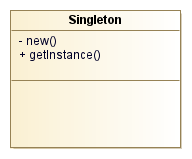
\includegraphics[width=0.5\textwidth]{singleton}
\end{figure}
\subparagraph{Abstract Factory}
Contexto: Debemos crear diferentes objetos, todos pertenecientes a la misma familia. Por ejemplo: las bibliotecas para crear interfaces gráficas suelen utilizar este patrón y cada familia sería un sistema operativo distinto. Así pues, el usuario declara un Botón, pero de forma más interna lo que está creando es un BotónWindows o un BotónLinux, por ejemplo.\\
El problema que intenta solucionar este patrón es el de crear diferentes familias de objetos.\\
El patrón Abstract Factory está aconsejado cuando se prevé la inclusión de nuevas familias de productos, pero puede resultar contraproducente cuando se añaden nuevos productos o cambian los existentes, puesto que afectaría a todas las familias creadas\\
\begin{figure}[h!]
  \centering{}
    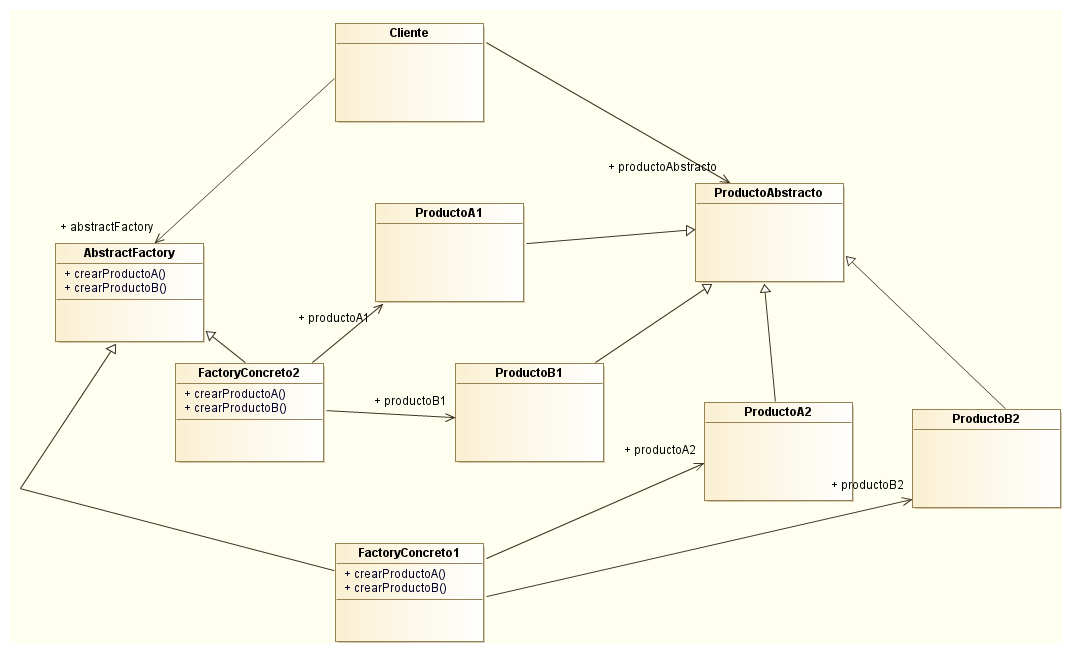
\includegraphics[width=1\textwidth]{abstract_factory}
\end{figure}
\newpage
\subparagraph{Factory Method}
El patrón de diseño Factory Method consiste en utilizar una clase constructora (al estilo del Abstract Factory) abstracta con unos cuantos métodos definidos y otro(s) abstracto(s): el dedicado a la construcción de objetos de un subtipo de un tipo determinado. Es una simplificación del Abstract Factory, en la que la clase abstracta tiene métodos concretos que usan algunos de los abstractos; según usemos una u otra hija de esta clase abstracta, tendremos uno u otro comportamiento.
\begin{figure}[h!]
  \centering{}
    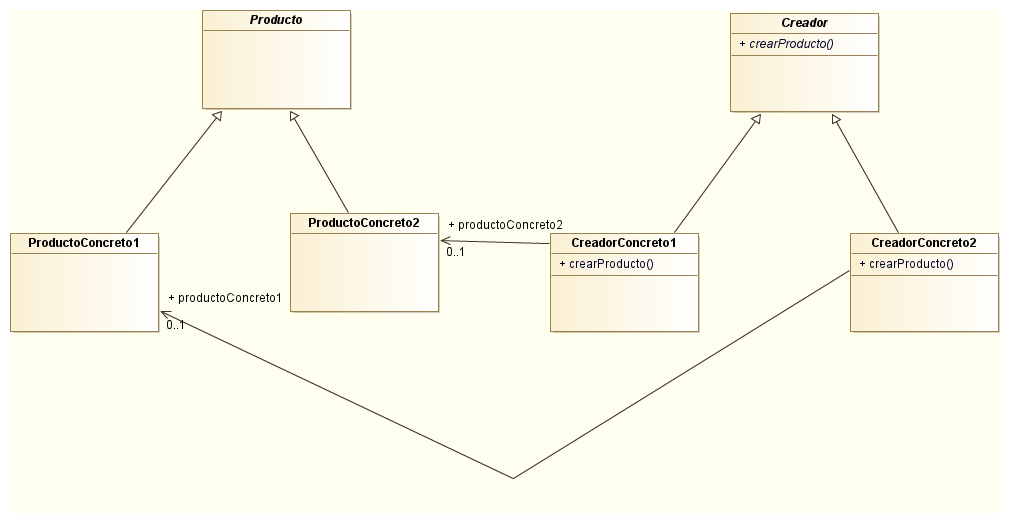
\includegraphics[width=1\textwidth]{factory_method}
\end{figure}
\subparagraph{Builder}
El patrón builder (Constructor) es usado para permitir la creación de una variedad de objetos complejos desde un objeto fuente (Producto), el objeto fuente se compone de una variedad de partes que contribuyen individualmente a la creación de cada objeto complejo a través de un conjunto de llamadas a interfaces comunes de la clase Abstract Builder.\\
Intención: Abstrae el proceso de creación de un objeto complejo, centralizando dicho proceso en un único punto, de tal forma que el mismo proceso de construcción pueda crear representaciones diferentes.\\
\begin{figure}[h!]
  \centering{}
    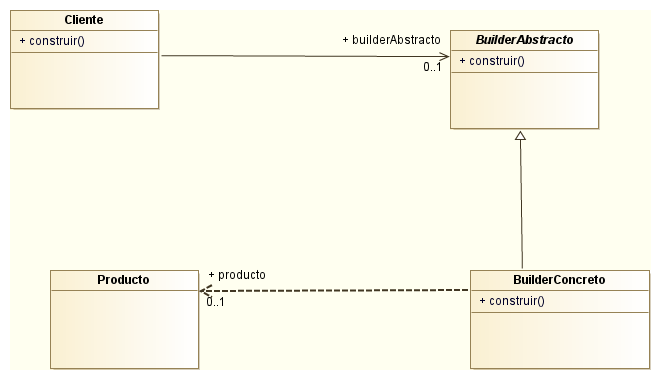
\includegraphics[width=1\textwidth]{builder}
\end{figure}
\subparagraph{Prototype}
El patrón de diseño Prototype (Prototipo), tiene como finalidad crear nuevos objetos duplicándolos, clonando una instancia creada previamente.\\
Este patrón especifica la clase de objetos a crear mediante la clonación de un prototipo que es una instancia ya creada. La clase de los objetos que servirán de prototipo deberá incluir en su interfaz la manera de solicitar una copia, que será desarrollada luego por las clases concretas de prototipos.
\begin{figure}[h!]
  \centering{}
    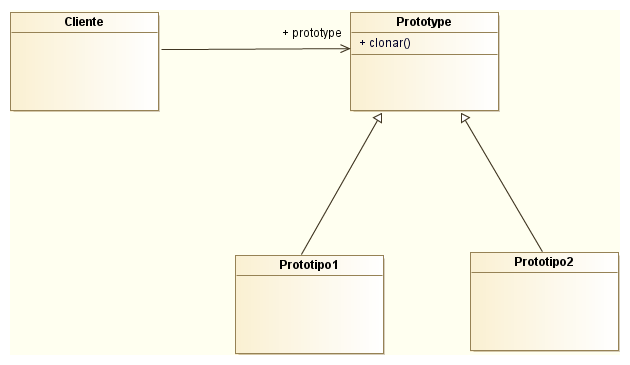
\includegraphics[width=1\textwidth]{prototype}
\end{figure}
\newpage
\paragraph{Patrones de Estructura}
\subparagraph{Adapter}
El patrón Adapter (Adaptador) se utiliza para transformar una interfaz en otra, de tal modo que una clase que no pudiera utilizar la primera, haga uso de ella a través de la segunda.
\begin{figure}[h!]
  \centering{}
    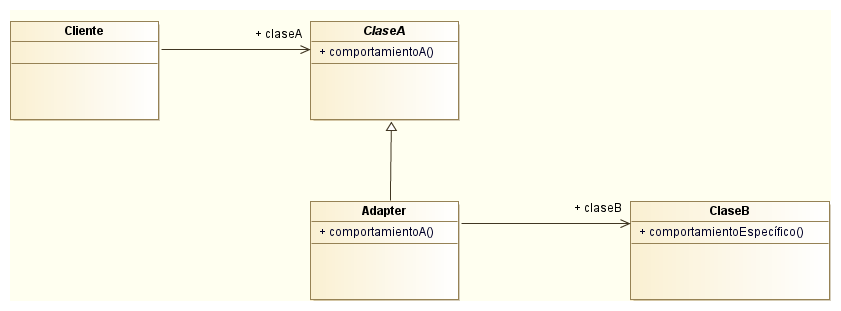
\includegraphics[width=1\textwidth]{adapter}
\end{figure}
\subparagraph{Bridge}
l patrón Bridge, también conocido como Handle/Body, es una técnica usada en programación para desacoplar una abstracción de su implementación, de manera que ambas puedan ser modificadas independientemente sin necesidad de alterar por ello la otra.\\
Esto es, se desacopla una abstracción de su implementación para que puedan variar independientemente.\\
\vspace*{\fill}
\noindent\makebox[\textwidth]{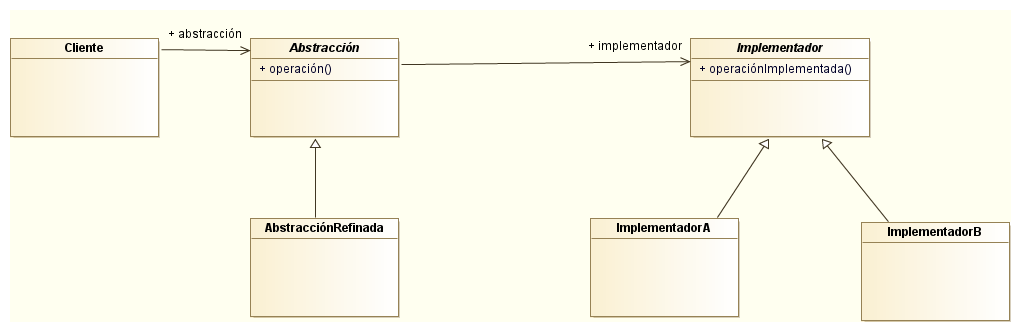
\includegraphics[width=1.2\textwidth]{bridge}}
\subparagraph{Composite}
El patrón Composite sirve para construir objetos complejos a partir de otros más simples y similares entre sí, gracias a la composición recursiva y a una estructura en forma de árbol.\\
Esto simplifica el tratamiento de los objetos creados, ya que al poseer todos ellos una interfaz común, se tratan todos de la misma manera.\\
\vspace*{\fill}
\noindent\makebox[\textwidth]{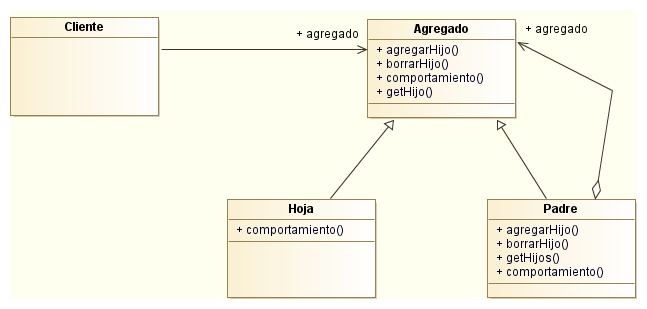
\includegraphics[width=1\textwidth]{composite}}
\subparagraph{Decorator}
El patrón Decorator responde a la necesidad de añadir dinámicamente funcionalidad a un Objeto. Esto nos permite no tener que crear sucesivas clases que hereden de la primera incorporando la nueva funcionalidad, sino otras que la implementan y se asocian a la primera.\\
\vspace*{\fill}
\noindent\makebox[\textwidth]{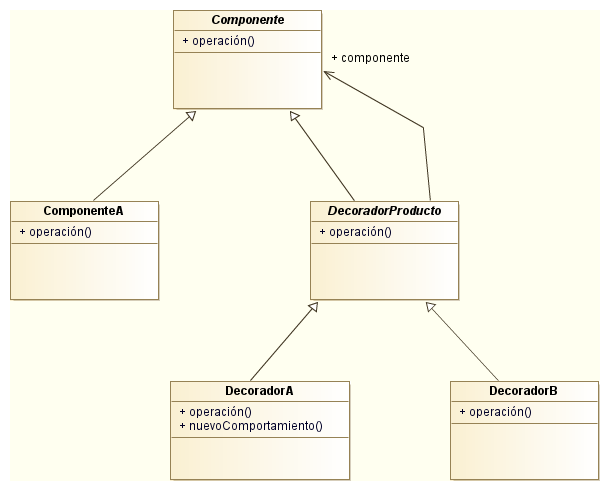
\includegraphics[width=1\textwidth]{decorator}}
\subparagraph{Facade}
El patrón fachada viene motivado por la necesidad de estructurar un entorno de programación y reducir su complejidad con la división en subsistemas, minimizando las comunicaciones y dependencias entre éstos.\\
Se aplicará el patrón fachada cuando se necesite proporcionar una interfaz simple para un subsistema complejo, o cuando se quiera estructurar varios subsistemas en capas, ya que las fachadas serían el punto de entrada a cada nivel. Otro escenario proclive para su aplicación surge de la necesidad de desacoplar un sistema de sus clientes y de otros subsistemas, haciéndolo más independiente, portable y reutilizable (esto es, reduciendo dependencias entre los subsistemas y los clientes).\\
\vspace*{\fill}
\noindent\makebox[\textwidth]{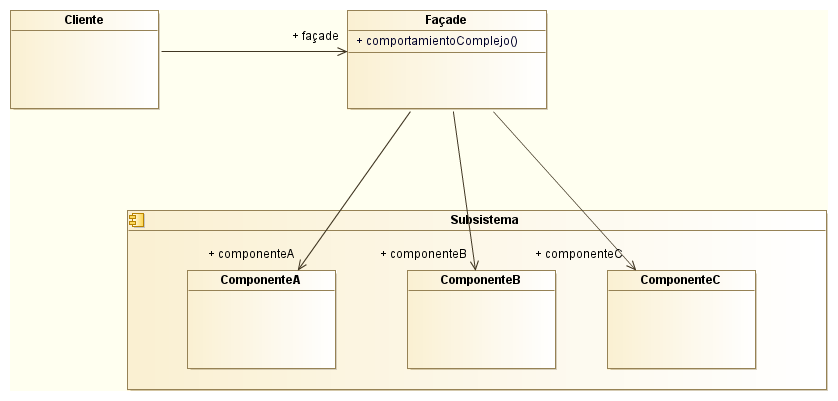
\includegraphics[width=1\textwidth]{facade}}
\subparagraph{Flyweight}
El patrón Flyweight (u objeto ligero) sirve para eliminar o reducir la redundancia cuando tenemos gran cantidad de objetos que contienen información idéntica, además de lograr un equilibrio entre flexibilidad y rendimiento (uso de recursos).\\
\vspace*{\fill}
\noindent\makebox[\textwidth]{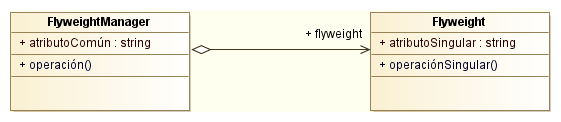
\includegraphics[width=1\textwidth]{flyweight}}
\subparagraph{Proxy}
El patrón Proxy es un patrón estructural que tiene como propósito proporcionar un subrogado o intermediario de un objeto para controlar su acceso.\\
\vspace*{\fill}
\noindent\makebox[\textwidth]{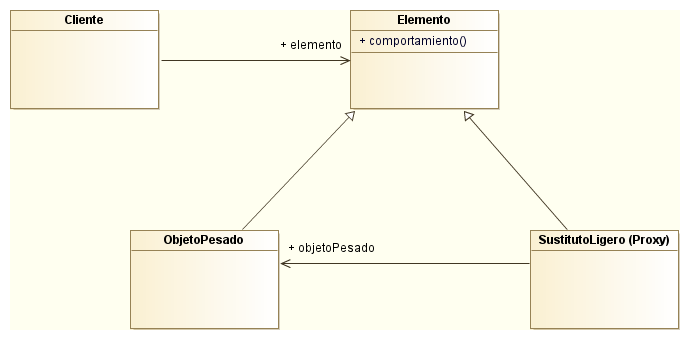
\includegraphics[width=1\textwidth]{proxy}}
\paragraph{Patrones de Comportamiento}
\subparagraph{Template Method}
Es un patrón de diseño enmarcado dentro de los llamados patrones de comportamiento, que se caracteriza por la definición, dentro de una operación de una superclase, de los pasos de un algoritmo, de forma que todos o parte de estos pasos son redefinidos en las subclases herederas de la citada superclase.\\
\vspace*{\fill}
\noindent\makebox[\textwidth]{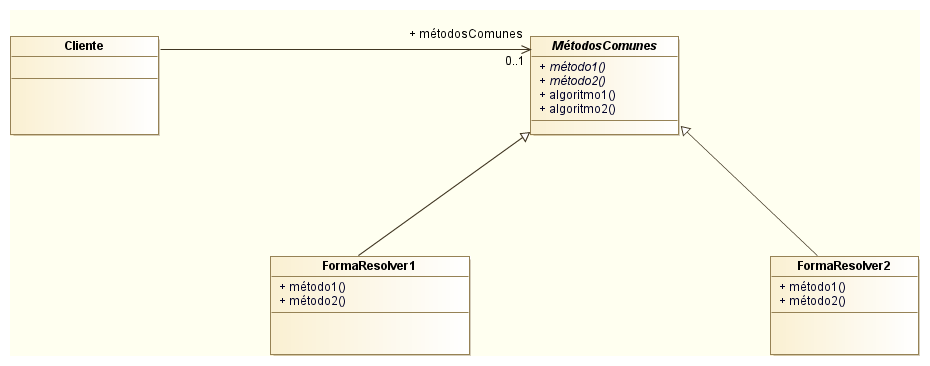
\includegraphics[width=1\textwidth]{template_method}}
\subparagraph{Chain of Responsability}
Es un patrón de comportamiento que evita acoplar el emisor de una petición a su receptor dando a más de un objeto la posibilidad de responder a una petición. Para ello, se encadenan los receptores y pasa la petición a través de la cadena hasta que es procesada por algún objeto. Este patrón es utilizado a menudo en el contexto de las interfaces gráficas de usuario donde un objeto puede contener varios objetos. Según si el ambiente de ventanas genera eventos, los objetos los manejan o los pasan.\\
\vspace*{\fill}
\noindent\makebox[\textwidth]{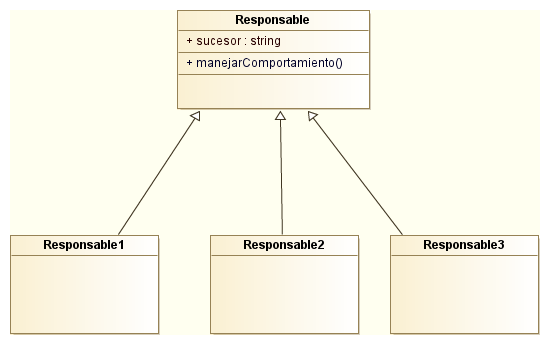
\includegraphics[width=1\textwidth]{chain_of_responsability}}
\subparagraph{Command}
Este patrón permite solicitar una operación a un objeto sin conocer realmente el contenido de esta operación, ni el receptor real de la misma. Para ello se encapsula la petición como un objeto, con lo que además se facilita la parametrización de los métodos.\\
\vspace*{\fill}
\noindent\makebox[\textwidth]{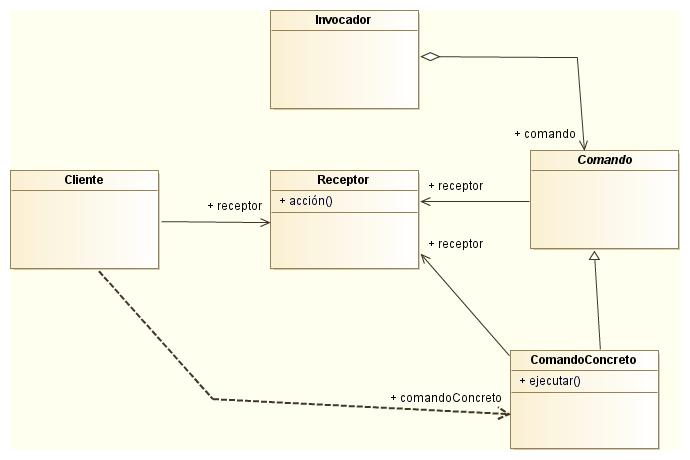
\includegraphics[width=1\textwidth]{command}}
\subparagraph{Iterator}
define una interfaz que declara los métodos necesarios para acceder secuencialmente a un grupo de objetos de una colección.\\
Este patrón de diseño permite recorrer una estructura de datos sin que sea necesario conocer la estructura interna de la misma.\\
\vspace*{\fill}
\noindent\makebox[\textwidth]{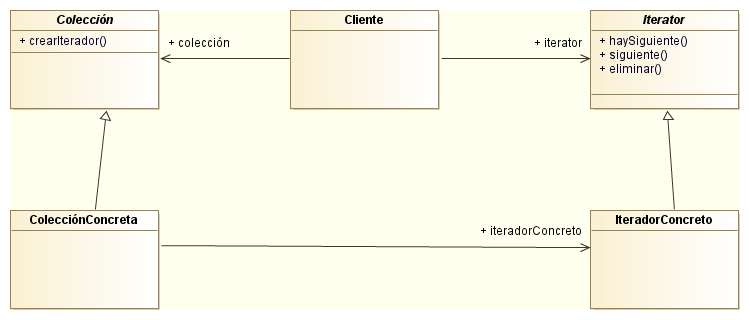
\includegraphics[width=1\textwidth]{iterator}}
\subparagraph{Mediator}
El patrón mediador define un objeto que encapsula cómo un conjunto de objetos interactúan. Este patrón de diseño está considerado como un patrón de comportamiento debido al hecho de que puede alterar el comportamiento del programa en ejecución.\\
\vspace*{\fill}
\noindent\makebox[\textwidth]{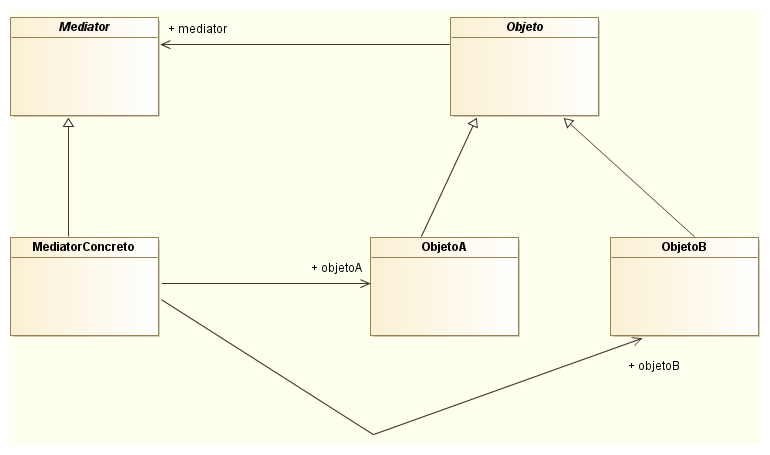
\includegraphics[width=1\textwidth]{mediator}}
\subparagraph{Memento}
Memento, es un patrón de diseño, cuya finalidad es almacenar el estado de un objeto (o del sistema completo) en un momento dado de manera que se pueda restaurar en ese punto de manera sencilla. Para ello se mantiene almacenado el estado del objeto para un instante de tiempo en una clase independiente de aquella a la que pertenece el objeto (pero sin romper la encapsulación), de forma que ese recuerdo permita que el objeto sea modificado y pueda volver a su estado anterior.\\
\vspace*{\fill}
\noindent\makebox[\textwidth]{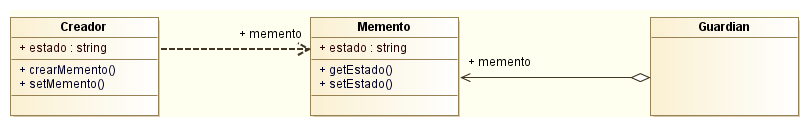
\includegraphics[width=1\textwidth]{memento}}
\subparagraph{Observer}
Definir una dependencia uno-a-muchos entre objetos, de tal forma que cuando el objeto cambie de estado, todos sus objetos dependientes sean notificados automáticamente. Se trata de desacoplar la clase de los objetos clientes del objeto, aumentando la modularidad del lenguaje, creando las mínimas dependencias y evitando bucles de actualización (espera activa o polling). En definitiva, normalmente, usaremos el patrón Observador cuando un elemento tiene que estar pendiente de otro, sin tener que estar encuestando de forma permanente si éste ha cambiado o no.\\
\vspace*{\fill}
\noindent\makebox[\textwidth]{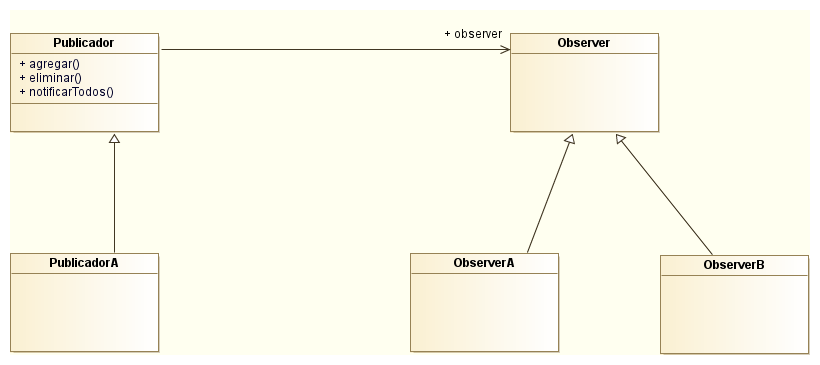
\includegraphics[width=1\textwidth]{observer}}
\subparagraph{State}
En determinadas ocasiones, cuando el contexto en el que se está desarrollando requiere que un objeto tenga diferentes comportamientos según el estado en que se encuentra, resulta complicado poder manejar el cambio de comportamientos y los estados de dicho objeto, todos dentro del mismo bloque de código. El patrón State propone una solución a esta complicación, creando básicamente, un objeto por cada estado posible del objeto que lo llama.\\
\vspace*{\fill}
\noindent\makebox[\textwidth]{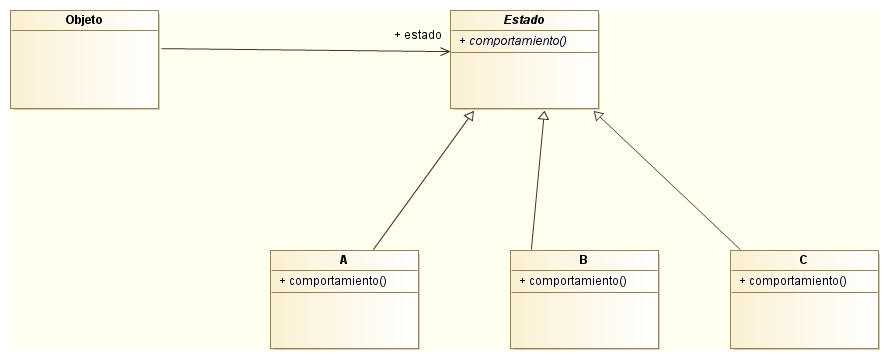
\includegraphics[width=1\textwidth]{state}}
\subparagraph{Strategy}
El patrón estrategia permite mantener un conjunto de algoritmos de entre los cuales el objeto cliente puede elegir aquel que le conviene e intercambiarlo dinámicamente según sus necesidades.\\
\vspace*{\fill}
\noindent\makebox[\textwidth]{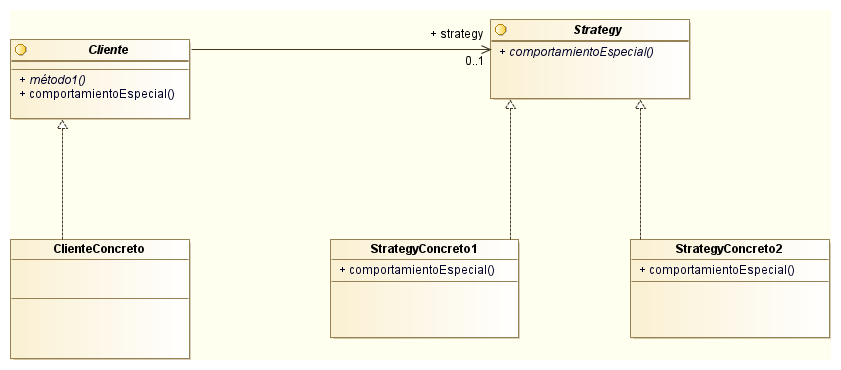
\includegraphics[width=1\textwidth]{strategy}}
\subsection{Mapeo de estructuras de clases a bases de datos relacionales}
\subsubsection{Problema de la impedancia}
En una base de datos relacional, la información se almacena en tablas. Los tipos a ser usados en las tablas son mayormente los tipos primitivos. Esto trae problemas al almacenar objetos.
\begin{itemize}
\item Los datos pueden almacenarse y no el comportamiento.
\item Solo los tipos de datos primitivos pueden almacenarse y no las estructuras complejas.
\end{itemize}
En vista de los problemas enunciados, necesitamos transformar nuestra estructura de información de objeto a una estructura orientada a tablas. Este problema se refiere a veces como el problema de la impedancia.\\
El problema de la impedancia trata aún otro problema: crea un fuerte acoplamiento entre la aplicación y el DBMS.\\
\subsubsection{Herencia}
Los objetos que deberían ser persistentes deberían ser mapeados en tablas de la base de datos. Se las clases se heredan unas a otras, hay principalmente dos maneras diferentes de resolver esto:
\begin{enumerate}
\item Los atributos heredados se copian a todas las tablas que representan las clases descendientes. Ninguna tabla representará la clase abstracta. \emph{Se elimina al ``padre''}.
\item La clase abstracta está en su propia tabla, a la que las tablas de las clases descendientes hacen referencia.
\end{enumerate}
¿Cuál alternativa es la mejor? No hay una mejor solución general para todos los casos, pero vamos a resaltar algunas de las propiedades de ambas alternativas. La primera es normalmente más rápida dado que no es necesario ningún joining o búsqueda en varias tablas para obtener información de un objeto.. Sin embargo, el tamaño de la base de datos aumentará dado que las columnas heredadas deben duplicarse. Además, si los cambios ocurren en los atributos heredados, los mismos afectarán a las tablas de todas las clases descendientes. En esta solución no tenemos ningún conocimiento de qué columnas se representan en la tabla que representa la clase abstracta. Una tabla específica que registre las diversas columnas sería entonces necesaria.\\
La segunda alternativa incluye menos redundancia, pero puede conducir a problemas si los identificadores son comunes en la tabla de la clase abstracta. Por ejemplo, si tenemos una clase abstracta persona; y estudiante y profesor son descendientes, entonces ninguna persona puede ser estudiante y profesor a la vez.
\subsection{Diseño de Interfaces de Usuario}
Para que un sistema alcance su potencial máximo es fundamental que su interfaz de usuario sea diseñada para ajustarse a las habilidades, experiencia y expectativas de sus usuarios previstos. Un buen diseño de la interfaz es crítico para la confiabilidad del sistema. Muchos de los llamados errores de usuario son causados por el hecho de que las interfaces de usuario no consideran las habilidades de los usuarios reales y su entorno de trabajo.\\
\subsubsection{Factores a tener en cuenta}
\begin{enumerate}
\item Las personas tienen una memoria limitada a corto plazo.
\item Todos cometemos errores, especialmente cuando tenemos que manejar demasiada información o estamos estresados.
\item Poseemos un amplio rango de capacidades físicas.
\item Tenemos diferentes preferencias de interacción.
\end{enumerate}
\subsubsection{Principios de diseño de interfaces gráficas}
\begin{center}
\begin{tabu}{p{7cm}|p{7cm}}
\rowfont{\bfseries\itshape\large} Principio & Descripción\\
\hline
\\[2pt]

Familiaridad de usuario. &
La interfaz debe utilizar términos y conceptos obtenidos de la experiencia de las personas que más utilizan el sistema.\\[2pt]
Uniformidad. &
Siempre que sea posible, la interfaz debe ser uiforme en el sentido de que las operaciones comparables se activen de la misma forma.\\[2pt]
Mínima sorpresa &
El comportamiento del sistema no debe provocar sorpresa a los usuarios.\\[2pt]
Recuperabilidad. &
La interfaz debe incluir mecanismos para permitir a los usuarios recuperarse de los errores.\\[2pt]
Guía de usuario. &
Cuando ocurran errores, la interfaz debe proporcionar retroalimentación significativa y características de ayuda sensible al contexto.\\[2pt]
Diversidad de usuarios. &
La interfaz debe proporcionar características de interacción apropiadas para los diferentes tipos de usuarios del sistema.
\end{tabu}
\end{center}

\subsubsection{Recursos de recuperación de errores}
\begin{enumerate}
\item Confirmación de acciones destructivas.
\item Proporcionar un recurso para deshacer.
\item Generar puntos de control.
\end{enumerate}
\subsubsection{Interacción del Usuario}
\begin{tabu}{|p{3cm}|p{3cm}|p{5cm}|p{3cm}|}
\hline
Estilos de Interacción &
Principales Ventajas &
Principales Desventajas &
Ejemplos de aplicación\\
\hline
Manipulación directa &
Interacción rápida e intuitiva. Fácil de aprender &
Puede ser difícil de implementar. Solo es adecuada donde existe una metáfora visual para las tareas y objetos &
Videojuegos y Sistemas CAD\\[2pt]
Selección de menús &
Evita errores del usuario. Se requiere teclear poco &
Lenta para usuarios experimientados. Puede llegar a ser compleja si existen muchas opciones en el menú &
La mayoría de los sistemas de propósito general\\[2pt]
Rellenado de formularios &
Introducción de datos sencilla &
Ocupa mucho espacio en laq pantalla. Causa problemas cuando las opciones del usuario no se ajustan a los campos del formulario &
Control de stock. Procesamiento de préstamos personales\\[2pt]
Lenguaje de comandos &
Poderoso y flexible &
Difícil de aprender. Gestión pobre de errores &
Sistemas operativos. Sistemas de comandos de control\\[2pt]
Lenguaje natural &
Accesible a usuarios casuales. Fácil de aplicar &
Se requiere teclear más. Los sistemas de comprensión de lenguaje natural no son fiables &
Sistemas de recuperación de información\\[2pt]
\hline
\end{tabu}
\subsubsection{Pautas para el uso del color}
\begin{center}
\begin{tabu}{p{7cm}|p{7cm}}
\rowfont{\bfseries\itshape\large} Factor & Descripción\\
\hline
\\[2pt]

Contexto &
Donde sea posible, los mensajes generados por el sistema deben reflejar el contexto actual del usuario. En lo posible el sistema debe ser consciente de lo que está haciendo el usuario y generar mensajes relacionados con su actividad.\\[2pt]
Experiencia &
Al aumentar la familiaridad de los usuarios con el sistema también se aumenta su molestia por los mensajes largos y significativos. Sin embargo, los principiantes tienen dificultades en comprender los mensajes cortos y concisos del problema. Se deben proporcionar ambos tipos de mensajes y permitir al usuario controlar la concisión de los mensajes.\\[2pt]
Nivel de habilidad &
Los mensajes se deben adaptar a las habilidades del usuario así como a su experiencia. \\[2pt]
Estilo &
Los mensajes deben ser positivos en vez de negativos. Deben estar escritos en modo activo y no en pasivo. No deben ser insultantes o tratar de ser graciosos.\\[2pt]
Cultura &
En la medida de lo posible, el diseñador de mensajes debe estar familiarizado con la cultura del país donde se vende el sistema. Existen distintas diferencias culturales entre Europa, Asia y América.

\end{tabu}
\end{center}
\subsubsection{El proceso de diseño de la interfaz de usuario}
Es un proceso iterativo donde los usuario interactúan con los diseñadores y prototipos de interfacz para decidir las características, organización, apariencia y funcionamiento de la interfaz de usuario. Existen tres actividades en este proceso:
\begin{description}
\item[Análisis del usuario] Se desarrolla una comprensión de las tareas que este realiza, su entorno de trabajo, etc.
\item[Prototipado del sistema] Se desarrollan prototipos del sistema y se los expone a los usuarios quienes pueden guiar la evolución de la misma.
\item[Evaluación de la interfaz] Se recopila información de las experiencias reales de los usuarios con la interfaz.
\end{description}
\subsubsection{Atributos de usabilidad}
\begin{center}
\begin{tabu}{p{7cm}|p{7cm}}
\rowfont{\bfseries\itshape\large} Atributo & Descripción\\
\hline
\\[2pt]

Aprendizaje &
¿Cuánto tiempo tarda un usuario nuevo en ser protivo con el sistema?\\[2pt]
Velocidad de funcionamiento &
¿Cómo responde el sistema a las operaciones de trabajo del usuario?\\[2pt]
Robustez &
¿Qué tolerancia tiene el sistema a los errores del usuario? \\[2pt]
Recuperación &
¿Cómo se recupera el sistema a los errores del usuario?\\[2pt]
Adaptación &
¿Está muy atado el sistema a un único modelo de trabajo?

\end{tabu}
\end{center}

\subsubsection{Las ocho reglas de Shneiderman}
\begin{enumerate}
\item Buscar siempre la coherencia
\item Permitir el uso de `shortcuts'
\item Dar realimentación de información
\item Diseñar diálogos que tengan un fin
\item Permitir manejos simples de los errores
\item Permitir deshacer las acciones con facilidad
\item Permitir que el centro de control sea interno
\item Reducir la carga de la memoria inmediata
\end{enumerate}

	\section{Diseño de Arquitecturas de Software}
\subsection{Diseño Arquitectónico}
\subsubsection{¿Qué es?}
Es la asignación de modelos de requerimiento esenciales a una tecnología específica. Es el plan del Diseño
\subsubsection{Proceso de Diseño Arquitectónico}
\begin{itemize}
	\item Determinar los requerimientos arquitectónicos.
	\item Diseño Arquitectónico.
	\item Validación.
\end{itemize}
\subsubsection{Rol del arquitecto}
\begin{itemize}
\item Revisa y negocia los requerimientos
\item Documentar la Arquitectura
\item Comunica la arquitectura, asegurándose que los involucrados comprendan.
\item Direcciona requerimientos no funcionales a la arquitectura
\item Configura la arquitectura de hardware
\item Se asegura que la arquitectura es respetada
\item Trabaja con el Administrador del Proyecto, ayudando en la planificación, la estimación la distribución de tareas y la calendarización del proyecto.
\end{itemize}
\subsubsection{Ventajas de diseñar y documentar la arquitectura}
\begin{itemize}
	\item Comunicación con los involucrados.
	\item Análisis del sistema.
	\item Reutilización a gran escala.
\end{itemize}
\subsubsection{Requerimiento no funcionales afectados por la arquitectura}
\begin{description}
	\item[Rendimiento] Si es un requerimiento crítico, la arquitectura debería diseñarse para identificar las operaciones críticas en un pequeño número de subsistemas con la mínima comunicación como sea posible entre ellas.
	\item[Protección] Si es un requerimiento crítico, debería usarse una arquitectura estructurada en capas, con las más crñiticas protegidas en capas más internas y aplicando una validación de seguridad de alto nivel en dichas capas.
	\item[Seguridad] Si es un requerimiento crítico, la arquitectura debería diseñarse para que las operaciones relacionadas con la seguridad se localizaran en un único subsistema o en un pequeño número de subsistemas.
	\item[Disponibilidad] Si es un requerimiento crítico, la arquitectura debería diseñarse para incluir componentes redundantes y para que sea posible reemplazar y actualizar componentes sin detener el sistema.
	\item[Mantenibilidad] Si es un requerimiento crítico, la arquitectura del sistema debería diseñarse usando componentes independientes de grano fino que puedan modificarse con facilidad.
\end{description}
\subsubsection{Conflictos arquitectónicos en requerimientos no funcionales}
\begin{itemize}
	\item Utilizar componentes de granularidad alta mejora la performance pero reduce mantenibilidad.
	\item La introducción de datos redundantes mejora la disponibilidad peor hace la seguridad más difícil.
	\item La localización de aspectos de seguridad relacionados usualmente significa más comunicación por lo tanto degrada la performance.
\end{itemize}
\subsubsection{Modelado de la Arquitectura}
El modelo arquitectónico mapea los requerimientos funcionales del análisis a una arquitectura tecnológica. Debe considerar información sobre:
\begin{itemize}
	\item Volúmenes de Datos.
	\item Funcionalidad más demandada en el negocio.
	\item Distribución geográfica.
	\item Distribución del Procesamiento de datos.
	\item Dónde se guardarán los datos.
	\item Cuáles procesos se ejecutarán en qué procesadores y que tanta comunicación se requerirá entre ellos.
\end{itemize}
\subsubsection{Salidas del Modelo Arquitectónico}
\begin{itemize}
	\item Distribución geográfica de los requerimientos de computación.
	\item Componentes de hardware para las máquinas clientes y para los servidores.
	\item Configuración y cantidad de niveles de hardware.
	\item Mecanismos y lenguajes de comunicación de la red.
	\item Sistema Operativo.
	\item Paradigma de Desarrollo.
	\item Lenguaje de Presentación (Front end)
	\item Lenguaje de fondo (back end)
	\item Sistema de Administración de Base de Datos.
	\item Ubicación/nes de los procesos.
	\item Ubicación/nes de los datos físicos.
	\item Estrategias de sincronización de los datos distribuidos físicamente.
\end{itemize}
\subsection{Patrones Arquitectónicos}
\subsubsection{Arquitectura Estratificada o en capas (Layered Style)}
Consiste en una pila de capas, donde cada capa actúa como máquina virtual de la capa de arriba. En un estilo estratificado simple, las capas sólo pueden usar la capa que está directamente debajo. La restricción significa que las capas subsiguientes más abajo están ocultas.
\paragraph{Calidad resultante}
La restricción del estilo trata directamente con los atributos de: modificabilidad, portabilidad, reusabilidad. Dado que las capas dependen sólo de la inmediata inferior las capas subsecuentes pueden ser intercambiadas o emuladas. Las capas superiores dan más oportunidades de sustitución frente a un posible problema de performance.
\paragraph{Ventajas}
\begin{itemize}
	\item Sustitución de capas completas en tanto se conserve la interfaz.
	\item En cada capa pueden incluirse facilidades redundantes para aumentar confiabilidad.
\end{itemize}
\paragraph{Desventajas}
\begin{itemize}
	\item Difícil mantener separación limpia entre capas y puede darse que capas de nivel superior se comuniquen con las de nivel inferior no adyacente.
	\item El rendimiento suele ser un problema, debido a múltiples niveles de interpretación de una solicitud de servicios mientras se procesa en cada capa.
\end{itemize}
\subsubsection{Arquitectura de Repositorio o Modelo Centrado}
\paragraph{Ventajas}
\begin{itemize}
	\item Los componentes pueden ser independientes, no necesitan conocer la existencia de otros componentes.
	\item Los cambios hechos por un componente se pueden propagar hacia todos los componentes.
	\item La totalidad de los datos se puede gestionar de manera consistente, centralizada, pues todos están en un lugar.
	\item Es extensible, se pueden agregar vistas y controladores más tarde, fácilmente.
	\item La concurrencia puede darse si vistas y controladores corren en sus propios hilos o procesos e incluso en hardwares diferentes.
\end{itemize}
\paragraph{Desventajas}
\begin{itemize}
	\item El repositorio es un punto de falla único, los problemas en el repositorio afectan a todo el sistema.
	\item Puede ser ineficiente al organizar la comunicación a través del repositorio.
	\item Difícil de distribuir en forma eficiente. Es posible distribuir un repositorio lógicamente centralizado, puede haber problemas con la redundancia e inconsistencia de los datos.
\end{itemize}
\subsubsection{Arquitectura Modelo-Vista-Controlador (MVC)}
\begin{itemize}
	\item Desacopla el modelo de las vistas estableciendo un modelo de suscripción/ notificación.
	\begin{itemize}
		\item La vista debe asegurarse que su apariencia refleja el estado del modelo.
		\item Frente a cambios el modelo se encarga de avisar a las vistas que dependen de él.
		\item La vista se actualiza a sí misma.
	\end{itemize}
	\item Se pueden crear varias vistas de un modelo, para ofrecer diferentes presentaciones.
\end{itemize}
\paragraph{Ventajas}
\begin{itemize}
	\item Permite que los datos cambien de manera independiente de su representación y viceversa.
	\item Soporte distintas representaciones de los mismos datos, y los cambios en una representación se muestran en todos ellos.
\end{itemize}
\paragraph{Desventajas}
Puede implicar código adicional y complejidad de código cuando el modelo de datos y las interacciones son simples.
\subsubsection{Arquitectura Publicar-Suscribir (Publish-Suscribe)}
\begin{itemize}
	\item Componentes independientes publican eventos y otros se suscriben a ellos.
	\item Los publicantes ignoran el motivo global por el cual el evento es publicado, los suscriptores ignoran porque o quien publica el evento y dependen sólo del evento no de quien lo publica.
	\item Cada tópico puede tener más de un publicante y los publicantes pueden aparecer y desaparecer dinámicamente, lo que le da flexibilidad sobre configuraciones estáticas.
	\item Los suscriptores pueden suscribirse y des-suscribirse dinámicamente a un tópico.
\end{itemize}
\paragraph{Ventajas}
\begin{itemize}
	\item El principal beneficio es desacoplar los componentes que producen los eventos de quienes los consumen, lo que hace la arquitectura mantenible y evolucionable.
	\item El bus de evento agrega una capa de indirección entre productores y consumidores, lo que podría dañar la performance del sistema. No obstante existen recursos reusables que hacen ajustes a la performance.
	\item Los canales (buses) de eventos varían en la propiedades que soportan.
\end{itemize}
\subsubsection{Arquitectura Comunicando (Messaging)}
\begin{itemize}
	\item Esta arquitectura desacopla emisores de receptores utilizando una cola
de mensajes intermedia.
	\item El emisor envía un mensaje al receptor y sabe que eventualmente será entregado, aunque la red esté caída o el receptor no esté disponible.
	\item El patrón tiene inherentemente bajo acoplamiento, esto promueve alta modificabilidad, dado que emisores y receptores no se conectan directamente.
	\item Los cambios en los formatos de los mensajes de los receptores pueden causar cambios en las implementaciones de los emisores.
	\item Los formatos de mensajes auto-descriptivos reducen esta dependencia.
\end{itemize}
\paragraph{Características}
\begin{itemize}
	\item El procesamiento de datos se organiza de forma que cada componente de procesamiento (filtro) sea discreto y realice un tipo de transformación de datos. Los datos fluyen (como en una tubería) de un componente a otro para su procesamiento.
	\item La característica clave es que la red completa de tuberías y filtros está continua e incrementalmente procesando datos.
	\item Aplica a elementos de tiempo de ejecución, es parte de la vista de ejecución (runtime)
	\item Se utiliza en aplicaciones de procesamiento de datos (tanto basadas en lotes [batch] como en transacciones, también puede usarse en software embebido.
\end{itemize}
\paragraph{Ventajas}
\begin{itemize}
	\item Fácil de entender y soporta reutilización de transformación.
	\item El estilo de flujo de trabajo coincide con la estructura de muchos procesos empresariales.
	\item La evolución al agregar transformaciones es directa.
	\item Puede implementarse como sistema secuencial o como uno concurrente.
\end{itemize}
\paragraph{Desventajas}
\begin{itemize}
	\item El formato para transferencia de datos debe acordarse entre las	transformaciones que se comunican.
	\item Cada transformación debe analizar sus entradas y sintetizar sus salidas al formato acordado.
	\item Esto aumenta la carga del sistema y dificulta la reutilización de transformaciones funcionales que usen estructuras de datos incompatibles.
	\item Son inapropiadas para aplicaciones interactivas.
\end{itemize}
\subsubsection{Arquitectura Lote-Secuencial (Batch-Sequential)}
\begin{itemize}
	\item Los datos fluyen de una etapa a otra y es procesado incrementalmente.
	\item A diferencia del Pipe \& Filter cada etapa completa todo su procesamiento antes de escribir su salida.
	\item Los datos fluyen entre etapas en una cadena, pero es más común escribir en un archivo o disco.
\end{itemize}
\subsubsection{Arquitectura Agente (Broker)}
\paragraph{Propiedades clave del patrón}
\begin{description}
	\item [Arquitectura Hub-and.spoke] El agente actúa como concentrador de mensajes y los remitentes y receptores se conectan como rayos. Las conexiones al agente son por medio de puertos asociados a un formato específico de mensaje.
	\item[Realiza ruteo de mensajes] El agente incrusta la lógica de procesamiento para entregar un mensaje recibido en un puerto de entrada en el puerto de salida. La entrega.
	\item[Realiza transformación de mensajes] El agente lógico transforma el tipo de mensaje de origen recibido en el puerto de entrada en el tipo de mensaje de destino requerido por el puerto de salida.
\end{description}
\subsubsection{Arquitectura Coordinador de Proceso (Process Coordinator)}
\begin{description}
	\item[Encapsulamiento de Proceso] El coordinador de proceso encapsula la secuencia de pasos necesarios para completar un proceso de negocio. La secuencia puede ser arbitrariamente compleja. El coordinador es un único de definición para el proceso de negocio, haciendo más fácil de comprender y modificar. Recibe un requerimiento de inicio de proceso, llama a los servidores en el orden definido por el proceso y emite los resultados.
	\item[Bajo Acoplamiento] Los componentes del servidor son inconscientes de su rol en el proceso de negocio general, y del orden de los pasos del proceso. Los servidores simplemente definen un conjunto de servicios que pueden ejecutar y el coordinador los llama cuando es necesario como parte del proceso de negocio.
	\item[Comunicaciones Flexibles] Las comunicaciones entre el coordinador y los servidores pueden ser sincrónicas o asincrónicas. Para las comunicaciones sincrónicas, el coordinador espera hasta que el servidor responda. Para las comunicaciones asincrónicas, el coordinador provee una llamada o respuesta cola/tópico, y espera hasta que el servidor responde utilizando.
\end{description}

\subsection{Vistas Arquitectónicas}
\subsubsection{Tipos de vistas}
\begin{description}
	\item[Tipo de Vista de Módulo] Contiene vistas de los elementos que se pueden ver en tiempo de compilación. Definiciones de tipos de componentes, puertos y conectores, clases e interfaces.
	\item[Tipo de Vista de Ejecución] Contiene vistas de los elementos que se pueden ver en tiempo de ejecución. Incluye escenarios de funcionalidad, listas de responsabilidad y ensambles de componentes. Instancias de componentes, conectores y puertos (como objetos).
	\item[Tipo de Vista de Distribución] Contiene vistas de elementos relacionados con la distribución del software en el hardware.
\end{description}
\subsubsection{Vistas en el PUD}
\begin{description}
	\item[Vistas de Diseño] Clases, interfaces, colaboraciones.
	\item[Vistas de implementación] Componentes.
	\item[Vista de Proceso] Clases Activas.
	\item[Vista de Despliegue] Nodos.
	\item[Vista de Funcionalidad] Vista de Casos de Uso.
\end{description}

	\section{Prueba del Sistema de Información}
\subsection{Pruebas de software}
\subsubsection{Conceptos generales}
La prueba es un proceso destructivo porque tenemos que indagar sobre lo que hicimos para detectar lo que hicimos mal.\\
Es conocido que la corrección de una falla provoca fallas adicionales, en consecuencia, si una falla aparece debemos probar todo el software.\\
La actividad de prueba puede normalmente dividirse en:
\begin{description}
	\item[Verificación] ¿Estamos construyendo el sistema \emph{correctamente}?
	\item[Validación] ¿Estamos construyendo el sistema correcto?
\end{description}
\subsubsection{Tipos de prueba}
\begin{description}
	\item[Test de Operación] Es el más común. El sistema es probado en operación normal.
	\item[Test de Escala Completa] Ejecutamos el sistema \emph{al máximo} con todos los equipos conectados y usados por muchos usuarios ejecutando casos de uso simultaneamente.
	\item[Test de Performance o de Capacidad] El objetivo de esta prueba es medir la capacidad de procesamiento del sistema.
	\item[Test de Sobrecarga] Cumple la función de determinar cómo se comporta el sistema cuando es \emph{sobrecargado}
	\item[Test Negativos] El sistema es sistemática e intencionalmente usado en forma incorrecta.
	\item[Test basados en requerimientos] Estas pruebas son las que pueden mapearse directamente desde la especificación de requerimientos.
	\item[Test Esgonómico] Son muy importantes si el sistema será usado por gente inexperta. Se prueban la consistencia de la interfaz, consistencia entre las interfaces de los distintos casos de uso, si los menús son lógicos y legibles y si se entienden los mensajes de falta.
	\item[Test de documentación de usuario] Se prueba la documentación del sistema.
	\item[Test de aceptación] Es ejecutado por la organización que solicita el sistema.
\end{description}
\subsubsection{Niveles de prueba}
\paragraph{Prueba de Unidad}
Involucra clases, bloques y paquetes de servicio. Consiste en:
\begin{description}
	\item[Prueba de Especificación o Caja Negra] Verifican el comportamiento de la interfaz de la unidad. \emph{Lo que hace} sin importar \emph{cómo}. Es importante no solo ver que se produzca una salida, sino que la misma sea correcta.
	\item[Prueba Estructural o de Caja Blanca] Se verifica si la estructura interna es la correcta.
	\item[Prueba Basada en estados] Prueba la interacción entre las operaciones de una clase, monitoreando los cambios que tienen lugar en los atributos de los objetos.
\end{description}
\paragraph{Pruebas de Integración}
Una vez que las unidades han sido certificadas en las pruebas, estas deberían integrarse en unidades más grandes y finalmente al sistema. El propósito de las pruebas de integración es determinar si las distintas unidades que han sido desarrolladas trabajan apropiadamente, juntas.\\
Las pruebas de integración se hacen probando cada caso de uso, uno a la vez desde dos puntos de vista:
\begin{description}
	\item[Uno interno] Basado en los diagramas de interacción.
	\item[Uno externo] Basado en las descripciones del modelo de requerimientos.
\end{description}
\paragraph{Prueba del Sistema}
Una vez que se han probado todos los casos de uso por separado se probará el sistema completo. Algunos casos de uso son ejecutados en paralelo y el sistema es sometido a diferentes cargas.
\subsection{Prueba en el Proceso Unificado de Desarrollo}
\subsubsection{Objetivo}
\begin{itemize}
	\item Planificar las pruebas necesarias en cada iteración.
	\item Diseñar e implementar las pruebas creanto los casos de prueba que especifican qué probar.
	\item Realizar las diferentes pruebas y manejar los resultados de cada prueba sistemáticamente.
\end{itemize}
\subsubsection{El papel de la prueba en el ciclo de vida del software}
La realización de pruebas se centra en las fases de elaboración, cuando se prueba la línea base ejecutable de la arquitectura y de construcción cuando el grueso del sistema está implementado. Duerante la fase de transición el centro se desplaza hacia la corrección de defectos durante los primeros usos y a las pruebas de regresión.
\subsubsection{Tipos de pruebas según el PDU}
\begin{description}
	\item[Pruebas de instalación] Verifican que el sistema puede ser instalado en la plataforma del cliente y que el sistema funcionará correctamente cuando sea instalado.
	\item[Pruebas de configuración] Verifican que el sistema funciona correctamente en diferentes configuraciones.
	\item[Pruebas negativas] Intentan provocar que el sistema falle para poder así revelar sus debilidades.
	\item[Peuebas de tensión] Identifican problemas con el sistema cuando hay recurso insuficientes.
\end{description}
\subsubsection{Artefactos}
\paragraph{Modelo de pruebas}
Describe principalmente cómo se prueban los componentes ejecutables en el modelo de implementación con pruebas de integración y de sistema.
\paragraph{Caso de prueba}
Especifica una forma de pribar el sistema, incluyendo la entreda o resultado con la que se ha de probar y condiciones. Casos de prueba comunes:
\begin{itemize}
	\item Caso de prueba que especifica cómo probar un caso de uso o un escenario específico de un caso de uso.
	\item Un caso de prueba que especifica cómo probar una realización de caso de uso de diseño o un escenario específico de una realización.
\end{itemize}
\paragraph{Procedimiento de prueba}
Especifica cómo realizar uno a varios casos de prueba o partes de estos.
\paragraph{Componente de prueba}
Automatiza uno o varios procedimientos de prueba o partes de ellos. Se utilizan para probar los componentes en el modelo de implementación.
\paragraph{Plan de prueba}
Describe estratégias, recursos y planificación de la prueba.
\paragraph{Defecto}
Es una anomalía del sistema.
\paragraph{Evaluación de la prueba}
Es una evaluación de los resultados de la prueba.
\subsubsection{Trabajadores}
\paragraph{Diseñador de pruebas}
Es responsable de la integridad del modelo de pruebas, asegurando que este cumple con su propósito. También planean las pruebas y seleccionan y describen los casos de pruebas y los procedimientos de prueba correspondientes que se necesitan.
\paragraph{Ingeniero de componentes}
Son responsables de los componentes de prueba que automatizan algunos de los procedimientos de prueba.
\paragraph{Ingeniero de pruebas de integración}
Son responsables de realizar las pruebas de  integración que se necesitan para cada construcción producida en el flujo de trabajo de la implementación.
\paragraph{Ingeniero de pruebas de sistema}
Es responsable de realizar las pruebas de sistema necesarias sobre una construcción que muestra el resultado de una iteración completa.
\subsubsection{Actividades}
\paragraph{Planificar la prueba}
El propósito de esta actividad es planificar los esfuerzos de prueba en una iteración llevando a cabo las siguientes tareas:
\begin{itemize}
	\item Describir una estratégia de pruebas.
	\item Estimar los requisitos para el esfuerzo de la prueba.
	\item Planificar el esfuerzo de la prueba.
\end{itemize}
\paragraph{Diseñar la prueba}
Los propósitos de esta actividad son:
\begin{itemize}
	\item Identificar y describir los casos de prueba para cada construcción.
	\item Identificar y estructurar los procedimientos de prueba especificando cómo realizar los casos de prueba.
\end{itemize}
\paragraph{Implementar una prueba}
El propósito de esta actividad es automatizar los procedimientos de prueba creando componentes de prueba si esto es posible.
\paragraph{Realizar pruebas de integración}
En esta actividad se realizan las pruebas de integración necesarias para cada una de las construcciones creadas en una iteración y se recopilan los resultados de las pruebas.
\paragraph{Realizar prueba de sistema}
En esta actividad se realizan las pruebas de sistema necesarias en cada iteración y se recopilan sus resultados.
\paragraph{Evaluar la prueba}
El propósito de esta actividad es evaluar los esfuerzos de prueba en una iteración.

	\section{Despliegue del Sistema de Información}
\subsection{Problemática del Despliegue de software}
Los desarrolladores de software a veces declaran la victoria demasiado pronto. Se olvidan que lo que marca el desarrollo exitoso del sistema es la disposición del cliente a usar el software terminado en vez de simplemente un software que compila satisfactoriamente.

	
	
\end{document}
